\documentclass[a4j,twocolumn]{jsarticle}

% 画像
\usepackage[dvipdfmx]{graphicx}
% 表
\usepackage{booktabs}
% 数式
\usepackage{amsmath}
% ベクトル
\usepackage{bm}
% コード
\usepackage{listings,jvlisting}
\usepackage{multicol}
% コードの色
\usepackage{color}
\definecolor{OliveGreen}{rgb}{0.0,0.6,0.0}
\definecolor{Orenge}{rgb}{0.89,0.55,0}
\definecolor{SkyBlue}{rgb}{0.28,0.28,0.95}
% ここからコードの表示に関する設定
\lstset{
  language=C,
  basicstyle={\ttfamily},
  identifierstyle={\small},
  commentstyle={\small\itshape},
  keywordstyle={\small\bfseries},
  ndkeywordstyle={\small},
  stringstyle={\small\ttfamily},
  frame={tb},
  breaklines=true,
  columns=[l]{fullflexible},
  numbers=left,
  xrightmargin=0zw,
  xleftmargin=3zw,
  numberstyle={\scriptsize},
  stepnumber=1,
  numbersep=1zw,
  lineskip=-0.5ex,
  keepspaces=true,
  keywordstyle={\color{SkyBlue}},
  commentstyle={\color{OliveGreen}},
  stringstyle=\color{Orenge},
  showstringspaces=false
}
\renewcommand{\lstlistingname}{Code}
% リンク
\usepackage[dvipdfmx]{hyperref}

\title{E1 前期実験考察 レポート}
\author{電気電子工学科 杉田太郎}
\date{\today}


\begin{document}

\maketitle

\section{はじめに}
$
\cdot E1実験では、平等電界の火花電圧がパッシェン曲線に沿うか、HPのデータを基に理論曲線を算出し、それを比較した。\\
\cdot また、グロー放電の電圧ー電流特性を測定した。\\
\cdot 不平等電解の火花電圧とコロナ電圧についても観察した。\\
\cdot 幾つかのグロー放電発酵をスペクトル分解して気体成分を同定した。\\
\cdot 窒素のSP02系列のスペクトルに注目することでそれの振動温度を求めた。\\
$



\section{検討課題}

\subsection*{平等電界の火花電圧}


図1は、球-球電極を使用し、圧力$p$及びギャップ長$d$を変化させて、火花電圧$V_s$を測定した。

ここで、ピラ二真空計で100Paを測定する際の注意点であるが、真空リークに注意しなければいけない。
また、1000Paを測定するときは、計測間隔が大きい1100Paから段々小さくしていくより、計測間隔がより小さい990Paから段々大きくしていくべきである。\\



$pd$が十分に大きいとき、火花電圧と$pd$は
$$V_S=E d=\frac{B p d}{\ln (A p d)-\ln \left[\ln \left(1+\frac{1}{\gamma}\right)\right]}$$
\cite{resnet1}
と式1で表すことができる。\\
(p:気圧[Torr],\\d:ギャップ長[cm],\\ A,B:定数,\\$\gamma$:陰極電極の状態で火花電圧$V_s$が変化すること)
ここに、A=20,B=365,$\gamma=0.005$を代入すると、

\begin{figure}[htb]
    \centering
    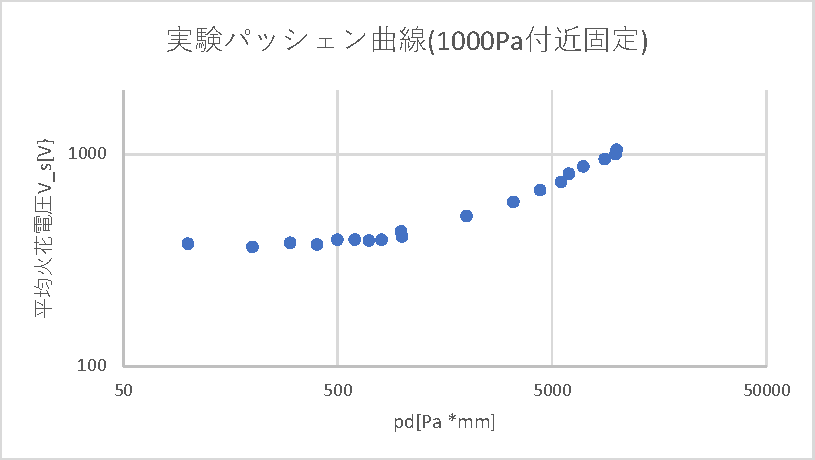
\includegraphics[keepaspectratio,width=0.6\columnwidth]{fig/zu1.pdf}
    \caption{実験でのパッシェン曲線}
\end{figure}

図1のようになる。この時、パッシェン曲線は連続に見えることから、$pd$の関数であることに納得できる。
(実際は、$\gamma$は定数ではないが、$pd$が十分に大きいとき、$\gamma$の変化は小さいことが推測できる。)

$pd$が十分に大きいときに火花電圧は$pd$の式で表せられることを確認できた。

\begin{figure}[htb]
    \centering
    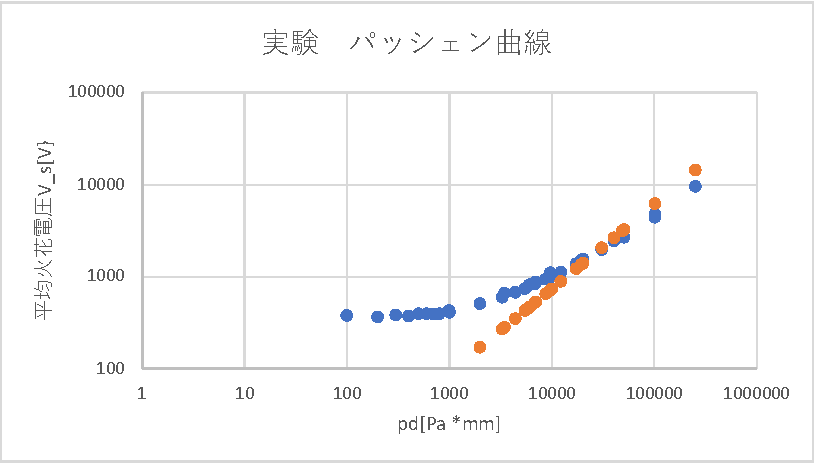
\includegraphics[keepaspectratio,width=0.6\columnwidth]{fig/zu2.pdf}
    \caption{実験でのパッシェン曲線(圧力を1000Pa付近固定)、青線:パッシェン曲線、橙線:式1}
\end{figure}


ここでの考察は、のちにパッシェン曲線の予測グラフを描画したときに後述する。
TODO

\subsection*{グロー放電の観測}

ガイスラー管の気圧を100(-120),667,2667Paで計測した。
その時の電圧ー電流特性は図3に示す。(電流ー電圧特性でないことに注意してください。)
また、100Paのように小さな気圧値では、どこかに空気漏れが発生してしまっていたことによって、
少しずつ外気が実験器具に入り込んでしまい、110,120Paになったのだと考える。
気圧が100Paのとき、電流ー電圧特性の関係は、直線の正の比例の関係にあると考えられる。
これは電圧を上げるほど、電子は加速されやすくなり、陰極から電子が放出される確率が上がるからと推測できる。
気圧が667Paのとき、電圧ー電流特性は、直線の負の比例の関係にあると見られるが、実験中の漏れから外気が入り込んでしまったことが原因だと考える。
気圧は2667Paは、測定できないが、気圧が大きいほど、同じ電流を流すのに必要とする電圧が大きいことがわかる。

\begin{figure}[htb]
    \centering
    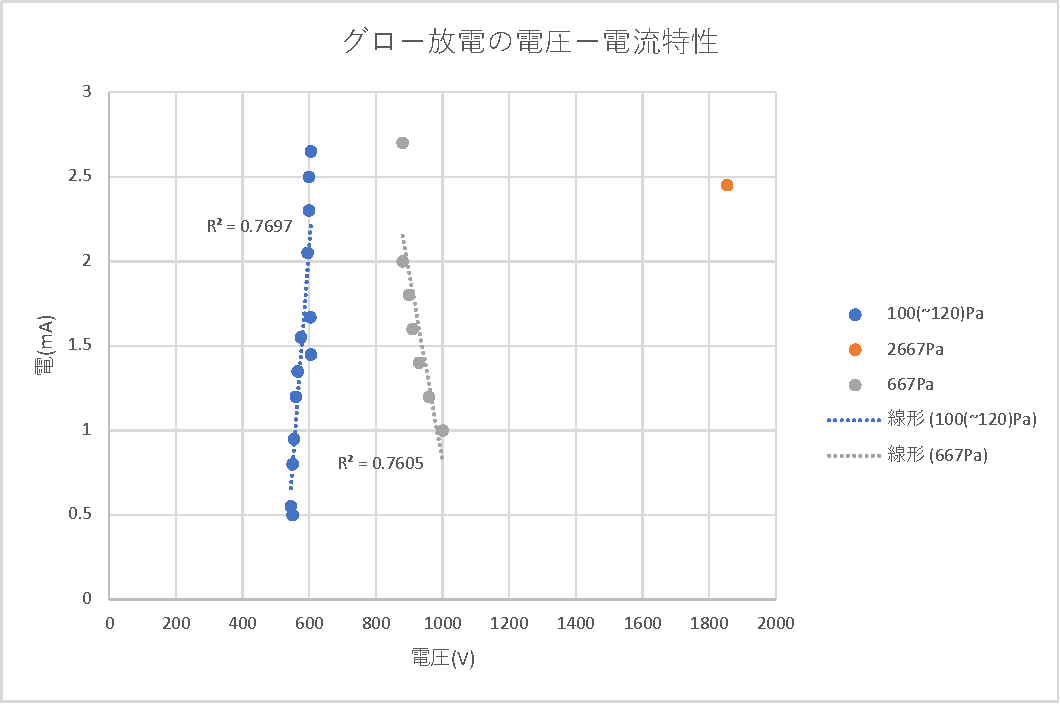
\includegraphics[keepaspectratio,width=0.8\columnwidth]{fig/glow.pdf}
    \caption{グロー放電の電圧ー電流特性}
\end{figure}

$
(ある電圧より上において図4のように正グローと融合してしまったため、それ以降は測定できなかった。)\\
\cdot 陰極暗部の厚さは、圧力が大きいほど、薄くなると思われた。
$

陰極暗部では、加速された電子が原子と電離反応を起こし、電子を雪崩方式で増やしていく反応が起きている。
ここで圧力が大きくなると空気中の原子が増えるので、電子はより短い距離を移動するだけで原子と衝突するようになる。
その結果、陰極暗部が小さくなると予想される。

\begin{figure}[htb]
    \centering
    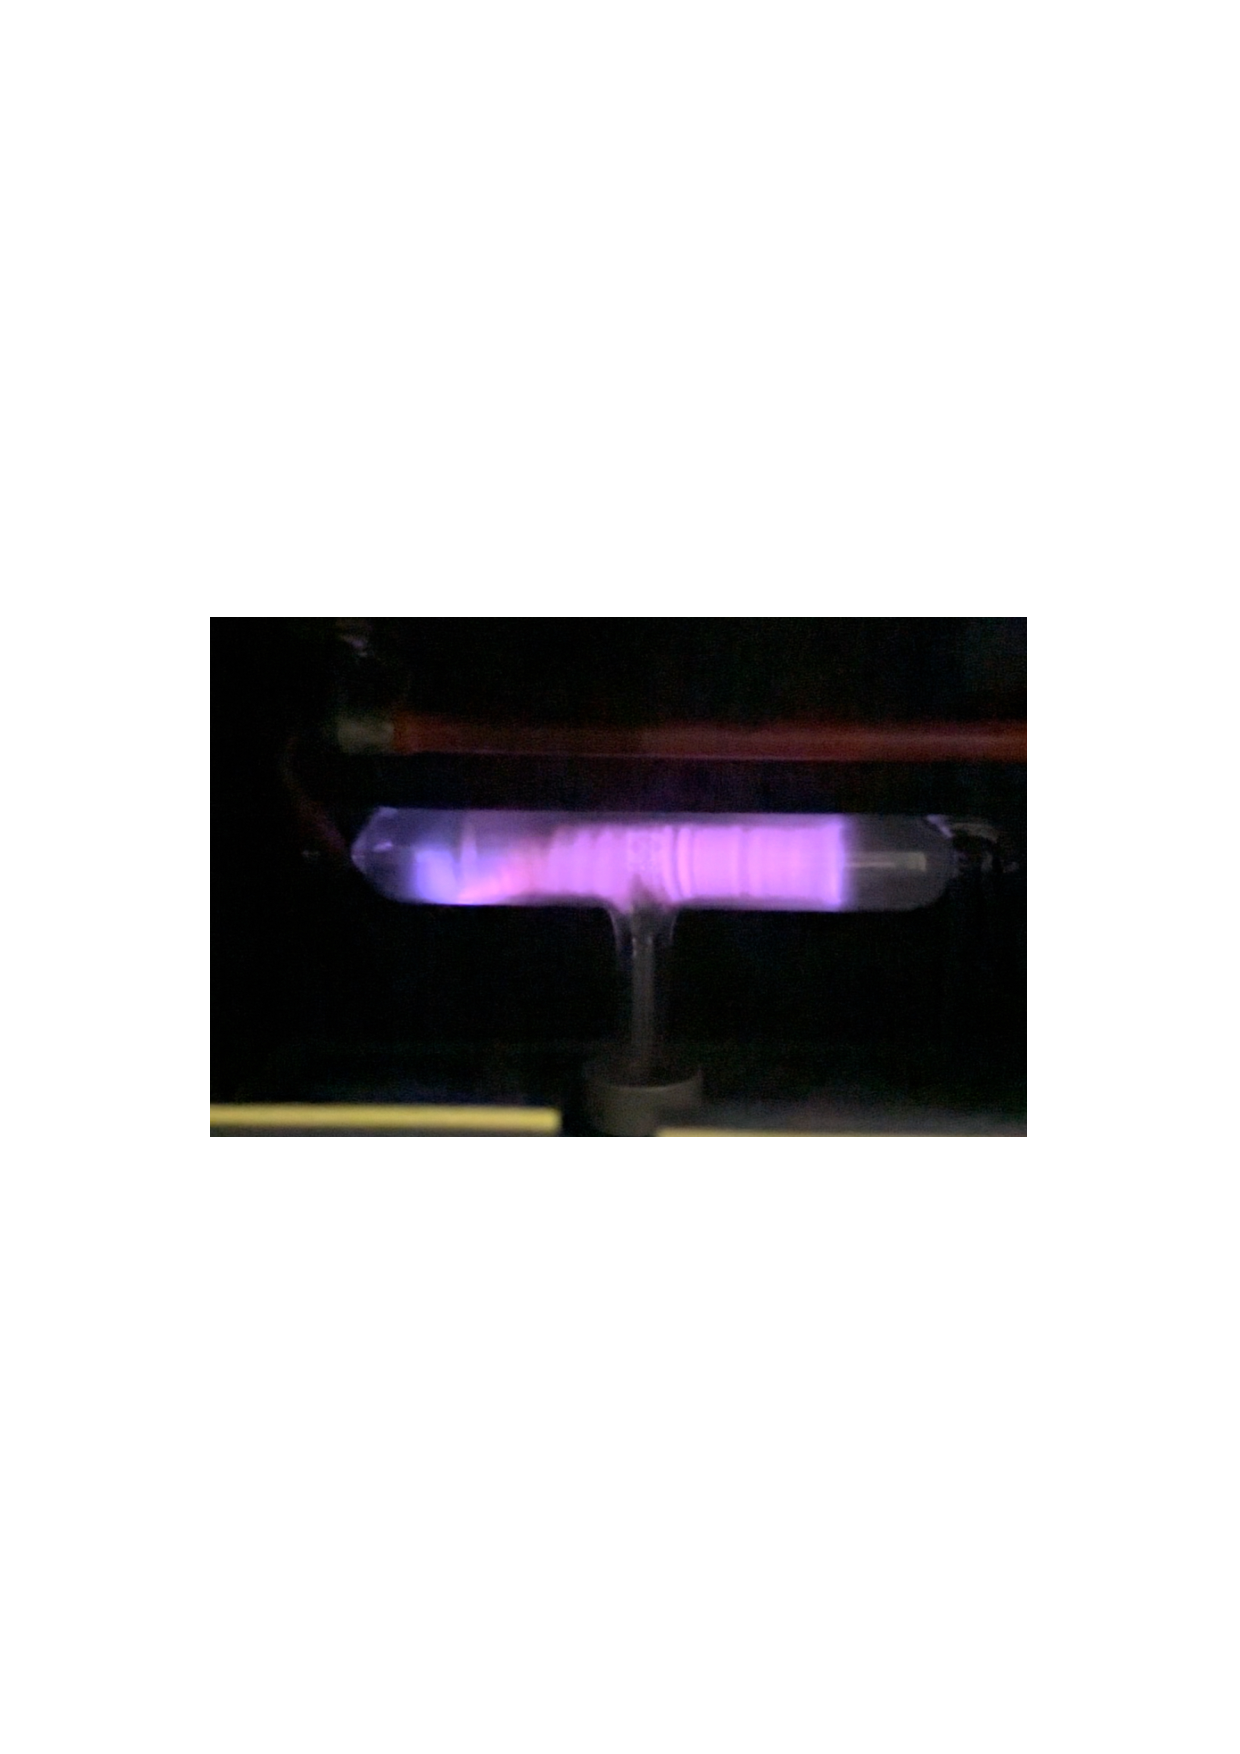
\includegraphics[keepaspectratio,width=0.6\columnwidth]{fig/fusion.pdf}
    \caption{正グローと負グローの様子}
\end{figure}


\subsection*{不平等電界の火花電圧と極性効果}

大気圧空気中で、円錐-平板電極の放電電圧のギャップ長特性を以下に図5-図7に示す。
正の直流電圧と交流電圧について、測定時間がなく、標本点不足により正確な電圧ー電流特性を測定できなかった。
この時、気温:23.8度、湿度:50.6$\%$、気圧は1018.5hPaであった。
また、図5のような電極形状にて実験が行われるため、極性効果について考える必要がある。
\begin{figure}[htb]
    \centering
    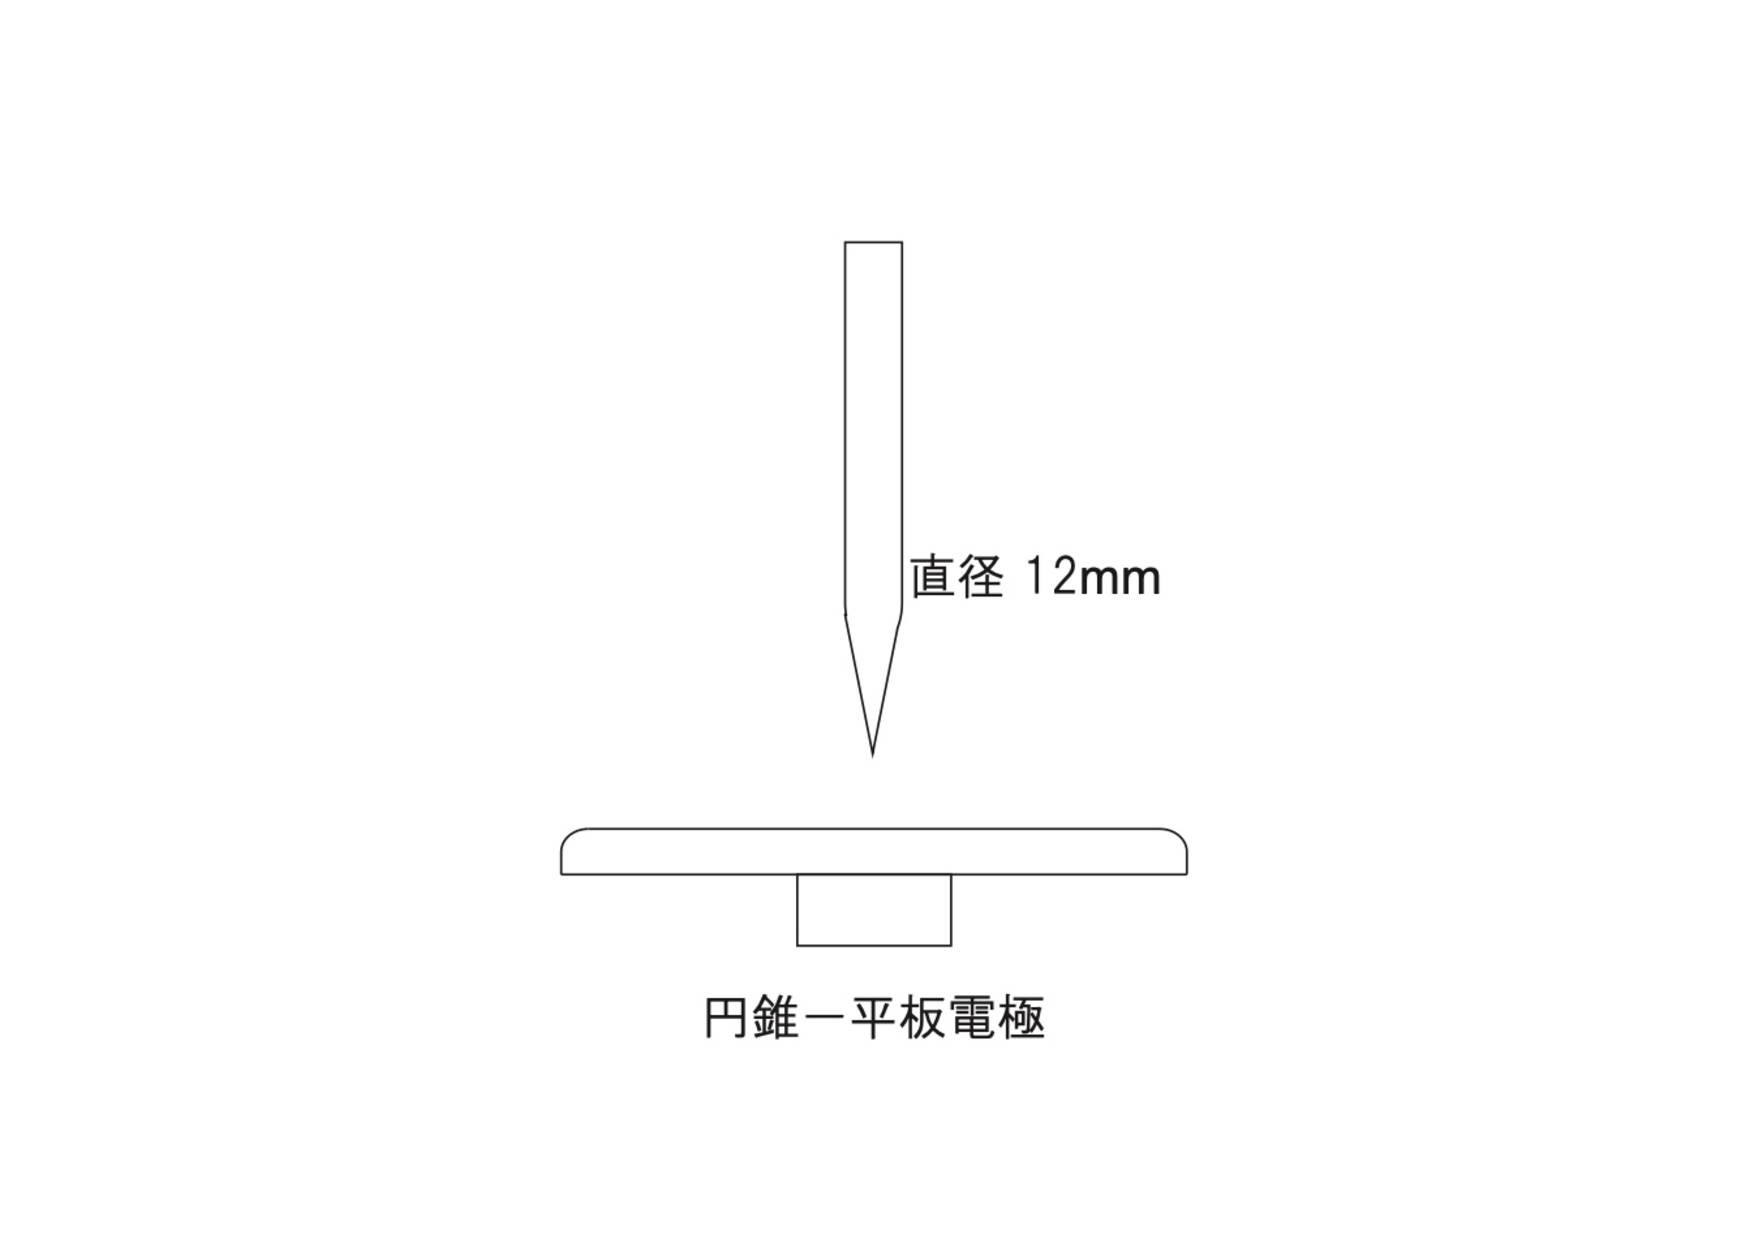
\includegraphics[keepaspectratio,width=0.6\columnwidth]{fig/pencil.pdf}
    \caption{不平等電界を作る電極形状}
    \cite{textbook}
\end{figure}

図5より、直流電圧は正より負であった方が、火花電圧において同一のギャップ長
において開始電圧が大きい。もし先が尖っている電極が正である場合、電子は加速され。空中で他の原子と衝突することで、
正イオンと新たな電子を形成し、また加速し原子と衝突を繰り返すことによって、雪崩のように、ギャップ中に電子と正イオンを作り出す。
この時、正イオンは陰極に衝突する際、陰極は平板であることから、真っ直ぐ陰極に加速し、$\gamma$効果によって、電子を出すことによって、持続的に火花を観測することができる。
一方、負である場合、正イオンは先が尖っている陰極の先端付近に集中してしまう。この場合、正イオンの衝突間隔の上昇、
陰極の先端の表面上の電子密度の低下によって、安定した火花のチャネルが形成されず、電圧が高くなってしまうことが考察される。\\

また、交流電圧の火花電圧は、直流電圧正火花電圧と値が近く、交流電圧の周波数は一連の衝突と電離の反応より十分に遅く、直流電圧負の状態では何も起きず、直流電圧正の状態において、
火花が開始されると推測できる。
TODOコロナ電圧について


雷インパルス電圧を印加した際、火花が発生するかどうかは、雷インパルス電圧が火花開始電圧を超えた時に、
自然電離電子がギャップ中に存在するかどうかである。したがって、火花が発生するかどうかは、確率的なものになるが、
正極性の雷インパルス電圧の方が負極性のものよりも火花が発生しやすいことが推測できる。



\begin{figure}[htb]
    \centering
    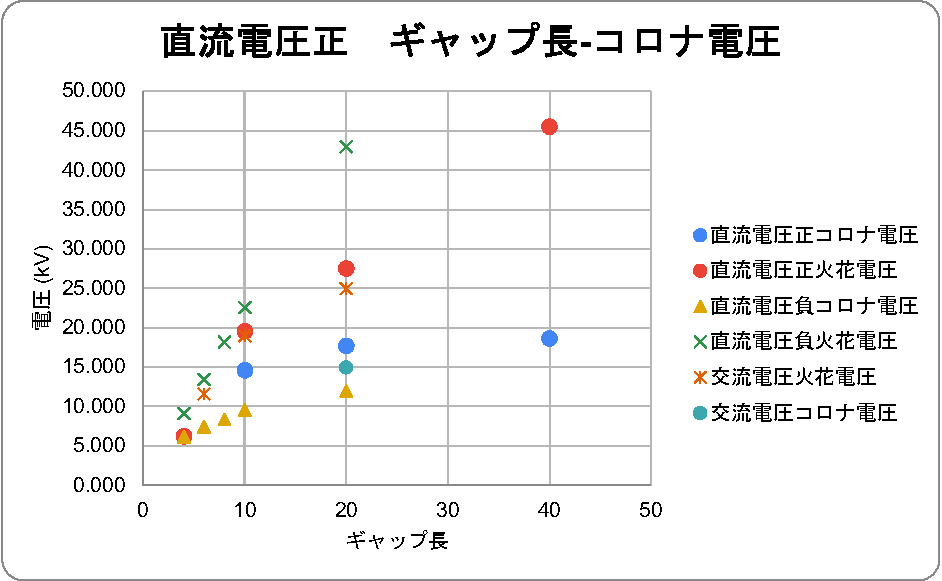
\includegraphics[keepaspectratio,width=0.6\columnwidth]{fig/disparity.pdf}
    \caption{交流電圧 ギャップ長-コロナ電圧}
\end{figure}



\subsection*{分光計測}
以下の図7-図12のように、それぞれの放電管内の気体を同定した。
また、中心と端で極端にスペクトルが異なったアルゴンとネオンもそれぞれ図13-14に示す。
また、プラズマボールは、ネオンとキセノンで構成されていると推測できる。
ネオン、キセノンのピーク値とプラズマボールのピーク値を元に、各元素の封入割合を計算すると、
キセノンが50.11$\%$、ネオンが49.89$\%$であることがわかり、ほぼ半分ずつ封入されていることがわかった。
この二つの元素はどちらも希ガスであり、極めて反応性が低いことから、安全性は高いと言える。

\begin{figure}[htb]
    \centering
    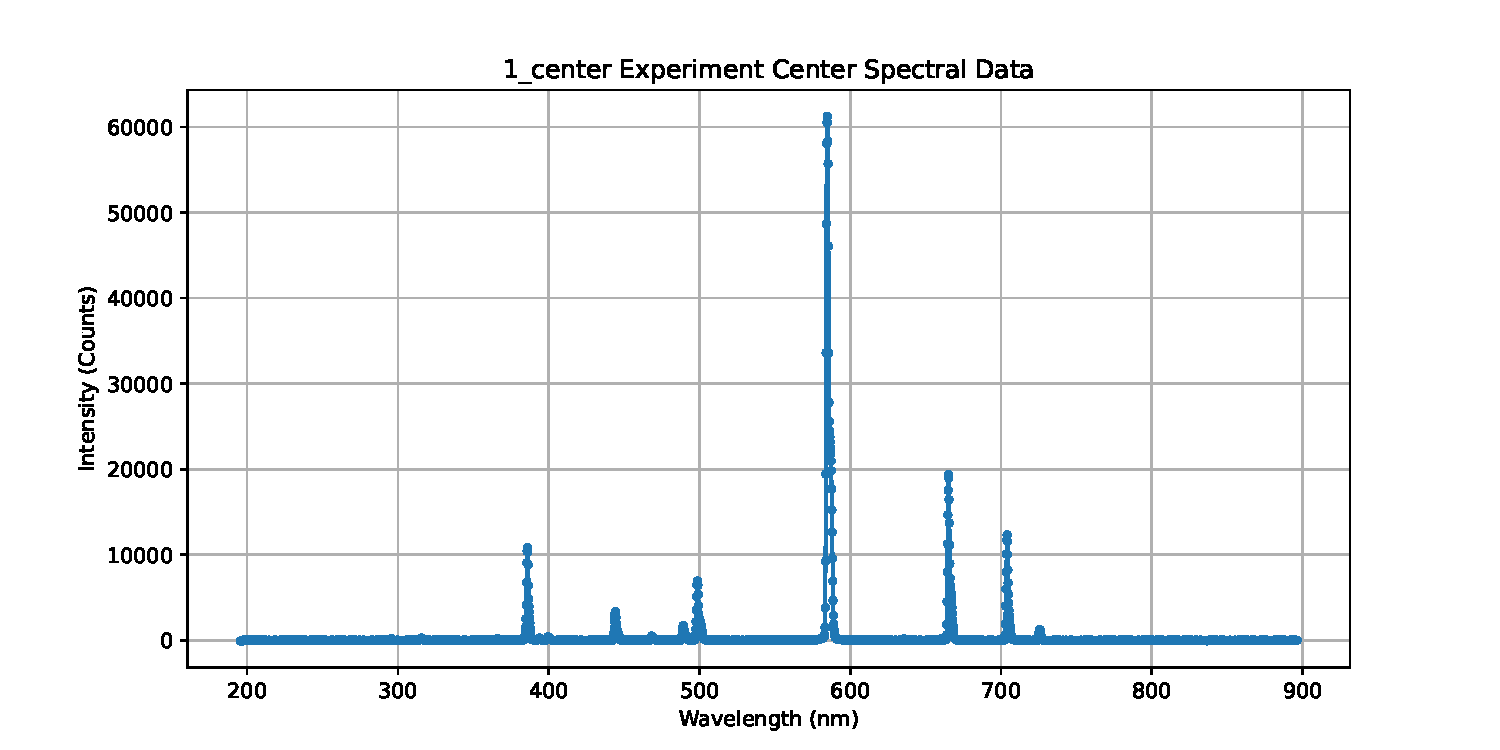
\includegraphics[keepaspectratio,width=0.6\columnwidth]{fig/1_center(He).pdf}
    \caption{$He$の中心のスペクトル}
\end{figure}
\begin{figure}[htb]
    \centering
    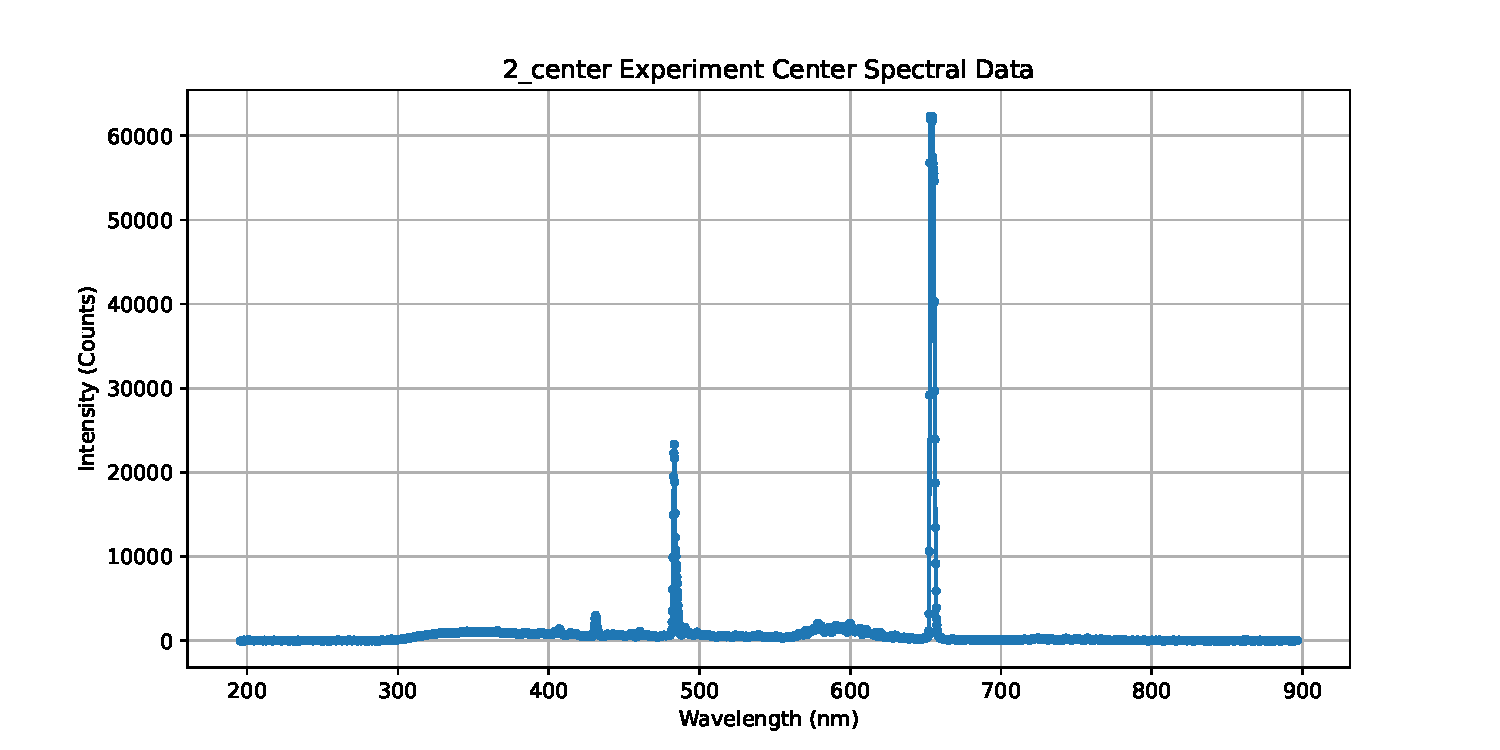
\includegraphics[keepaspectratio,width=0.6\columnwidth]{fig/2_center(H2).pdf}
    \caption{$H_2$の中心のスペクトル}
\end{figure}
\begin{figure}[htb]
    \centering
    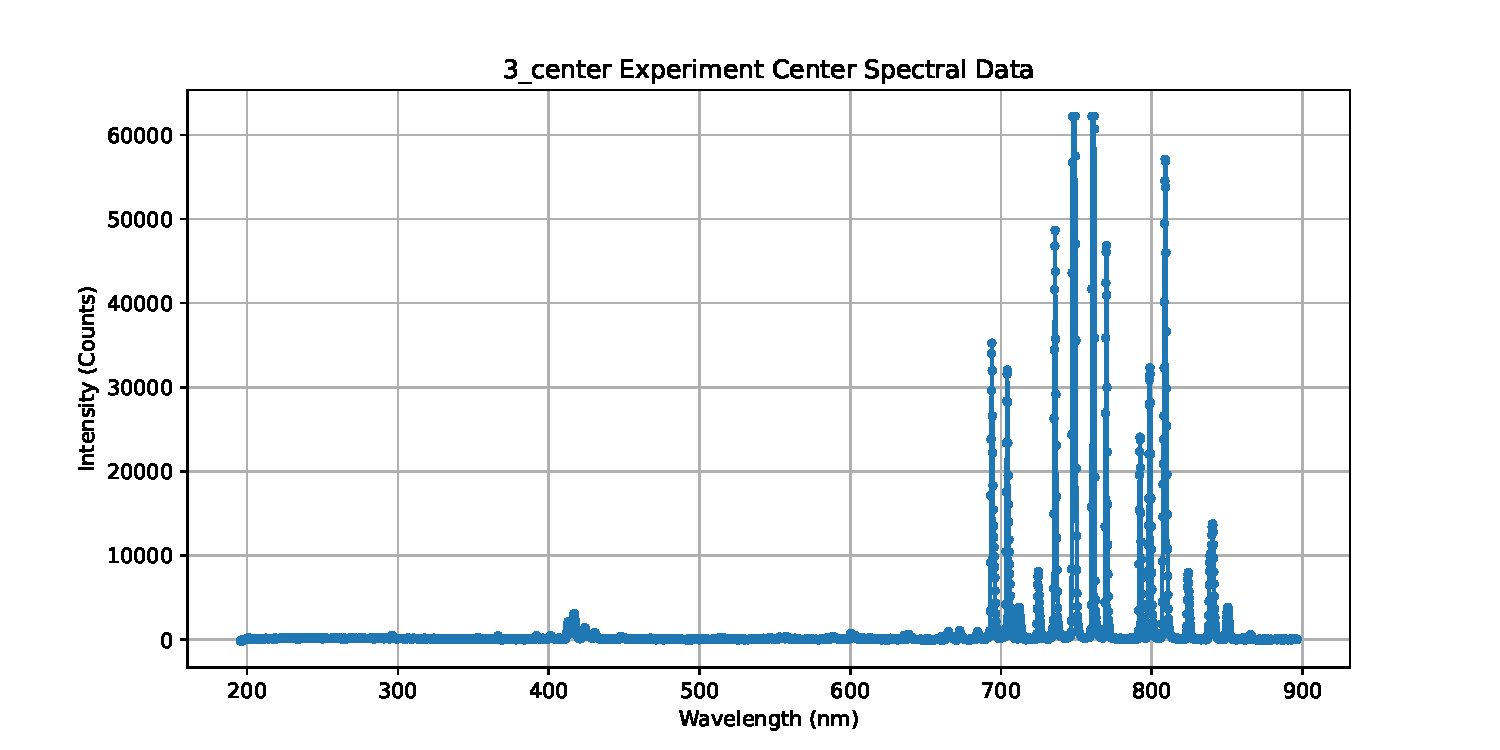
\includegraphics[keepaspectratio,width=0.6\columnwidth]{fig/3_center(Ar).pdf}
    \caption{$Ar$の中心のスペクトル}
\end{figure}
\begin{figure}[htb]
    \centering
    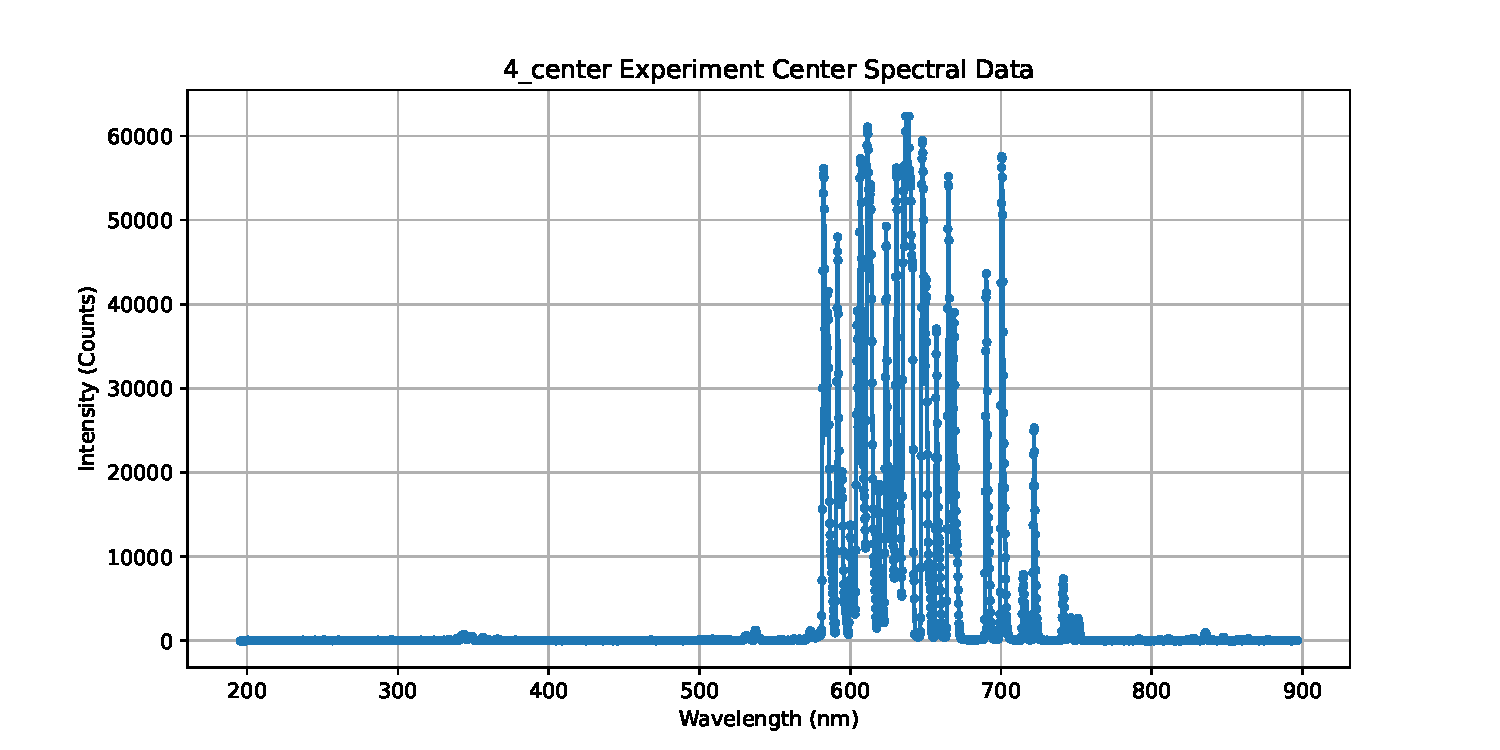
\includegraphics[keepaspectratio,width=0.6\columnwidth]{fig/4_center(Ne).pdf}
    \caption{$Ne$の中心のスペクトル}
\end{figure}
\begin{figure}[htb]
    \centering
    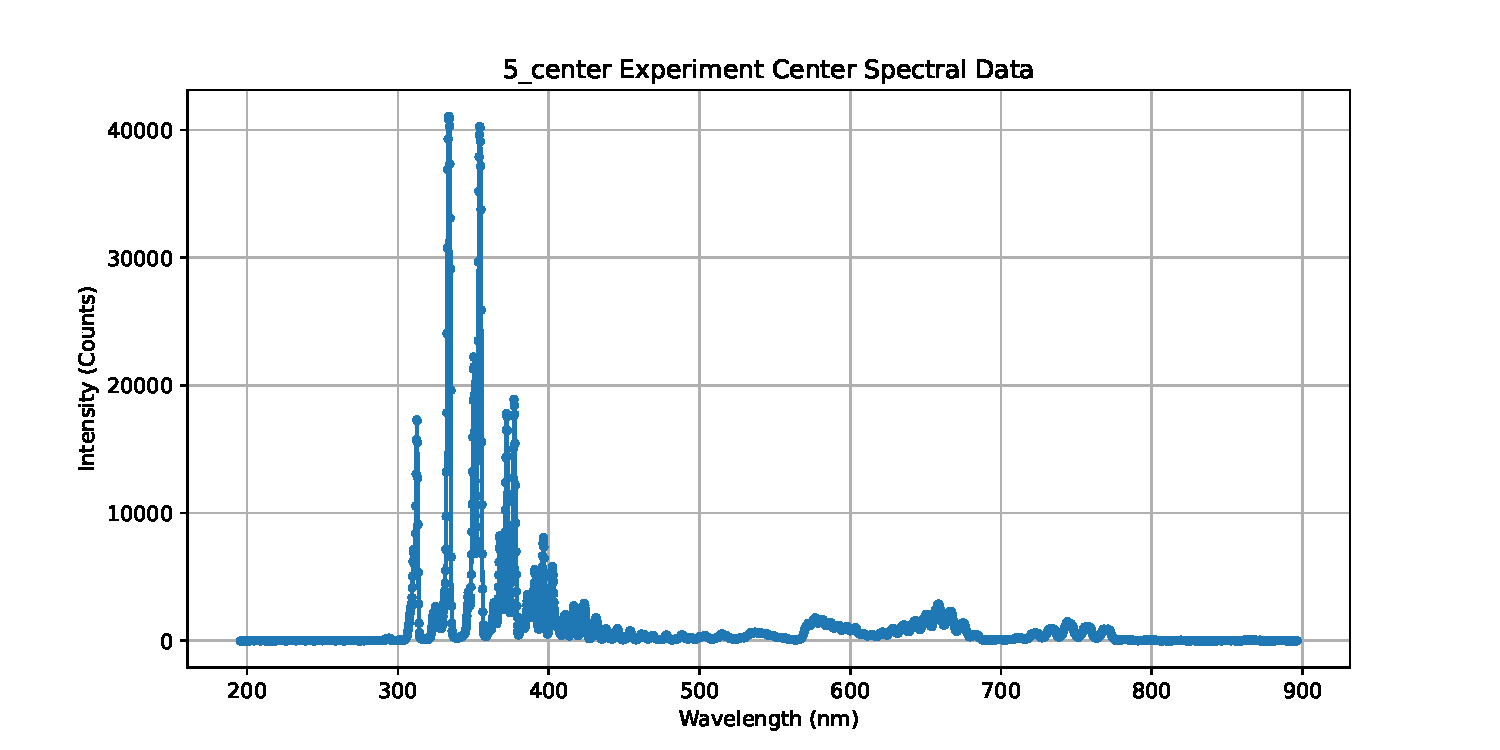
\includegraphics[keepaspectratio,width=0.6\columnwidth]{fig/5_center(N2).pdf}
    \caption{$N_2$の中心のスペクトル}
\end{figure}
\begin{figure}[htb]
    \centering
    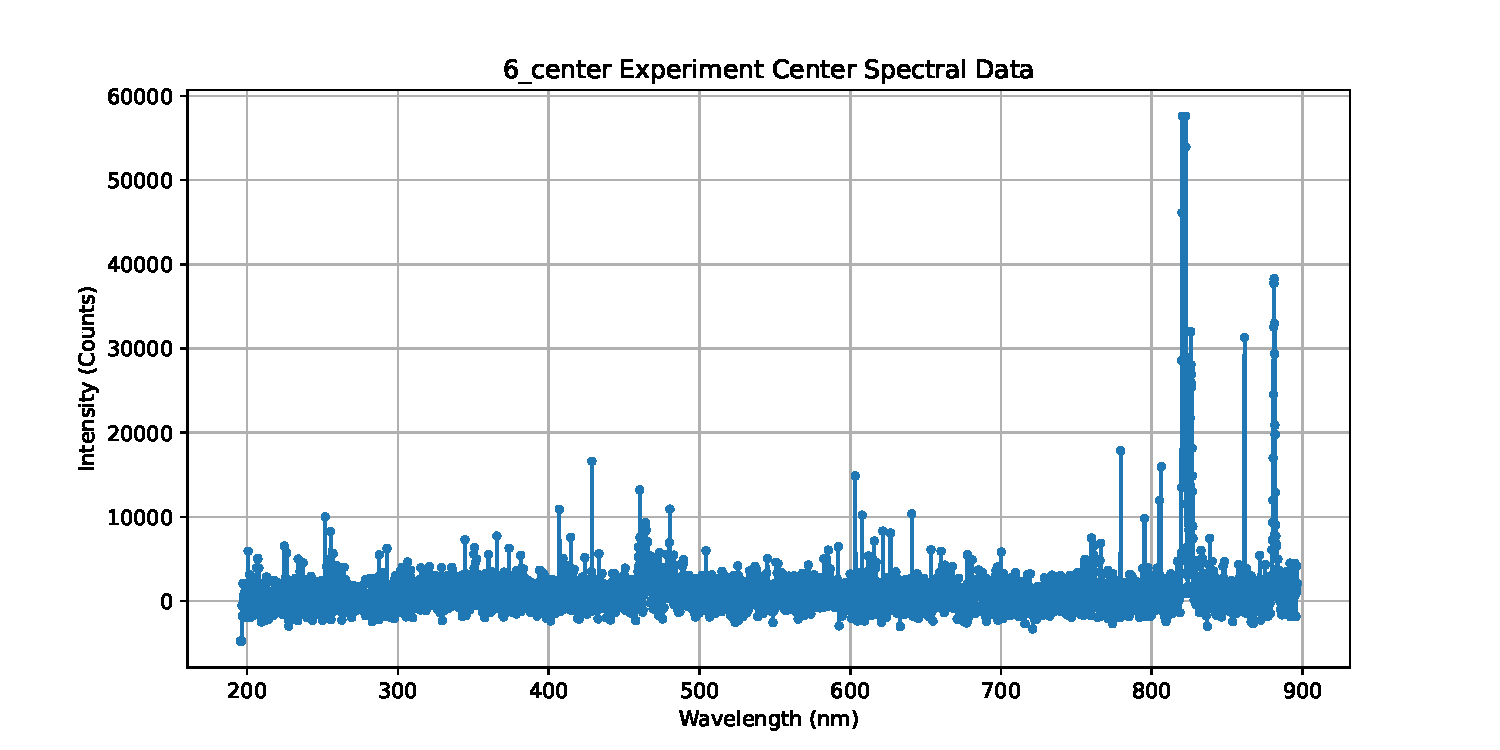
\includegraphics[keepaspectratio,width=0.6\columnwidth]{fig/6_center(Xe).pdf}
    \caption{$Xe$の中心のスペクトル}
\end{figure}

\begin{figure}[htb]
    \centering
    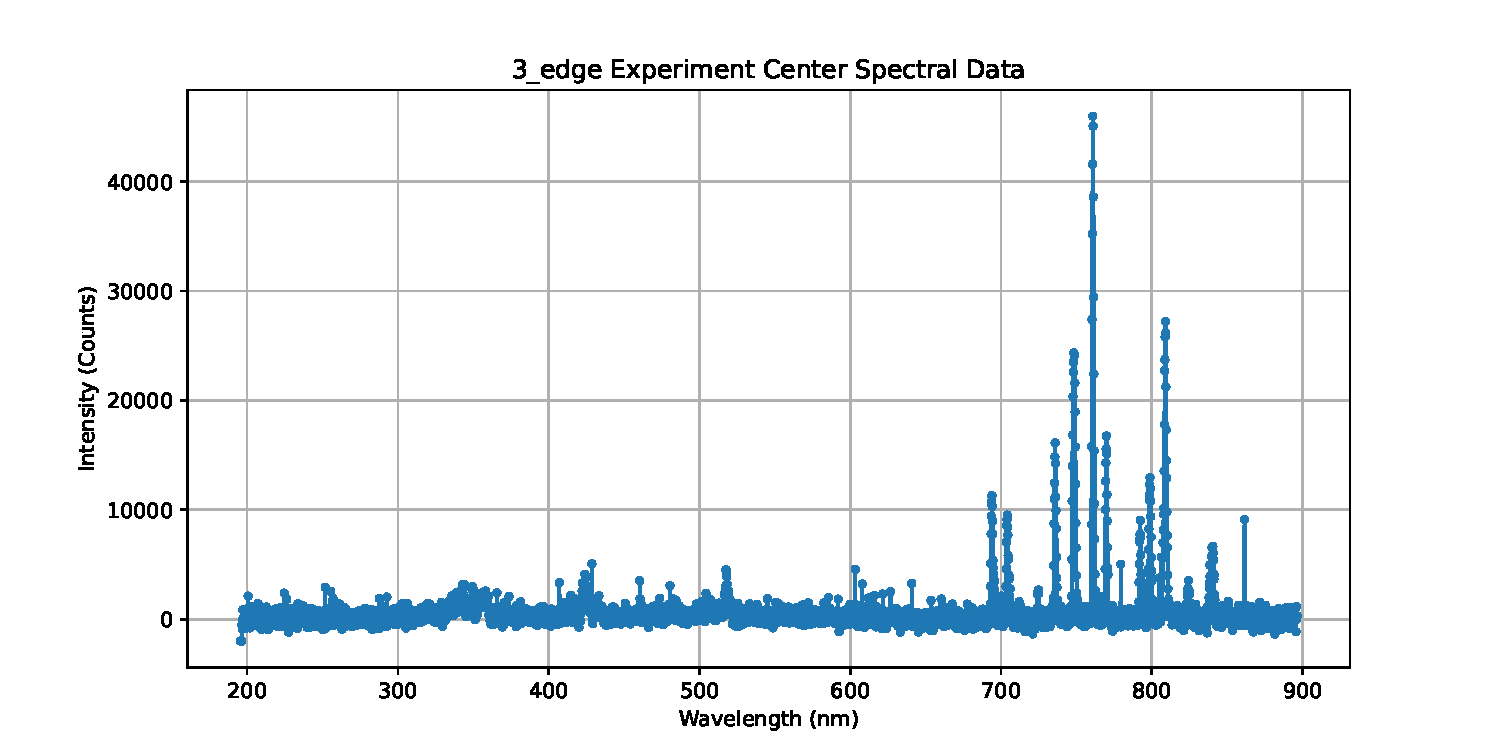
\includegraphics[keepaspectratio,width=0.6\columnwidth]{fig/3_edge(Ar).pdf}
    \caption{$Ar$の端のスペクトル}
\end{figure}
\begin{figure}[htb]
    \centering
    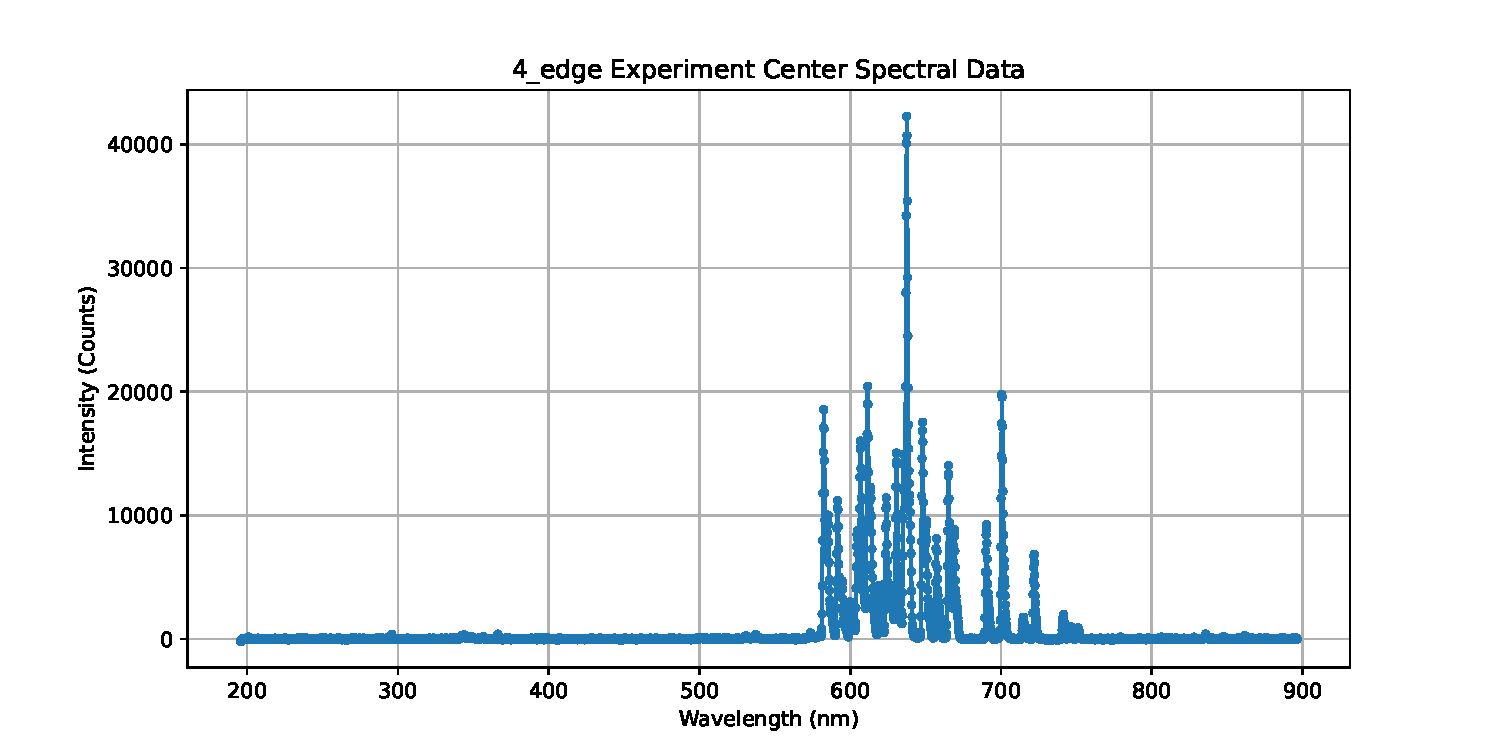
\includegraphics[keepaspectratio,width=0.6\columnwidth]{fig/4_edge(Ne).pdf}
    \caption{$Xe$の端のスペクトル}
\end{figure}

また、図15のようなカラーバーの7色の発光スペクトルを以下図16-図23に示す。
シアンは、緑+青。マゼンタは、赤+青。白は、赤+青+緑で構成されていると推測できる。
黒は全てのスペクトルを含んでいるとわかる。
\begin{figure}[htb]
    \centering
    
\includegraphics[keepaspectratio,width=0.6\columnwidth]{fig/color.pdf}
    \caption{カラーバー}
\end{figure}


\begin{figure}[htb]
    \centering
    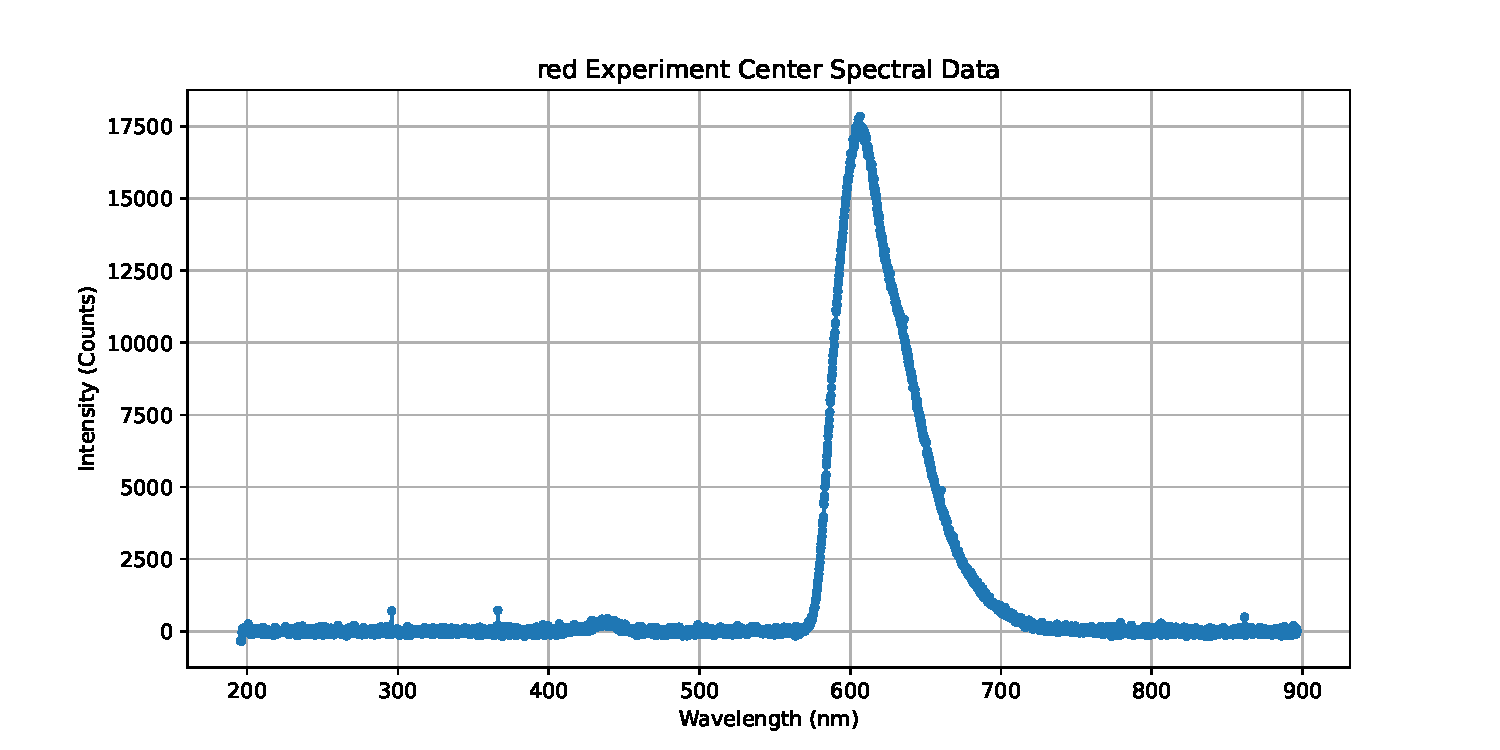
\includegraphics[keepaspectratio,width=0.6\columnwidth]{fig/red.pdf}
    \caption{赤のスペクトル}
\end{figure}
\begin{figure}[htb]
    \centering
    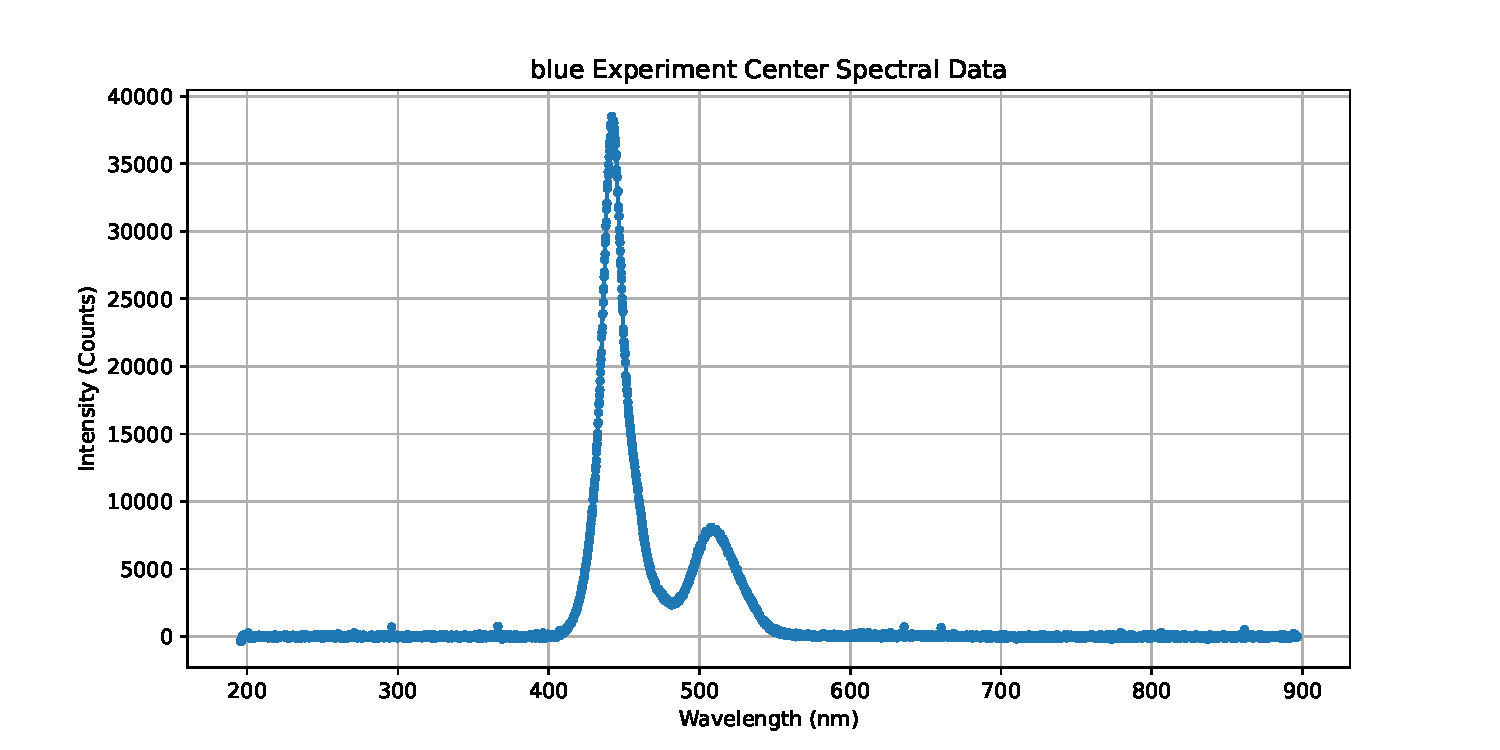
\includegraphics[keepaspectratio,width=0.6\columnwidth]{fig/blue.pdf}
    \caption{青のスペクトル}
\end{figure}
\begin{figure}[htb]
    \centering
    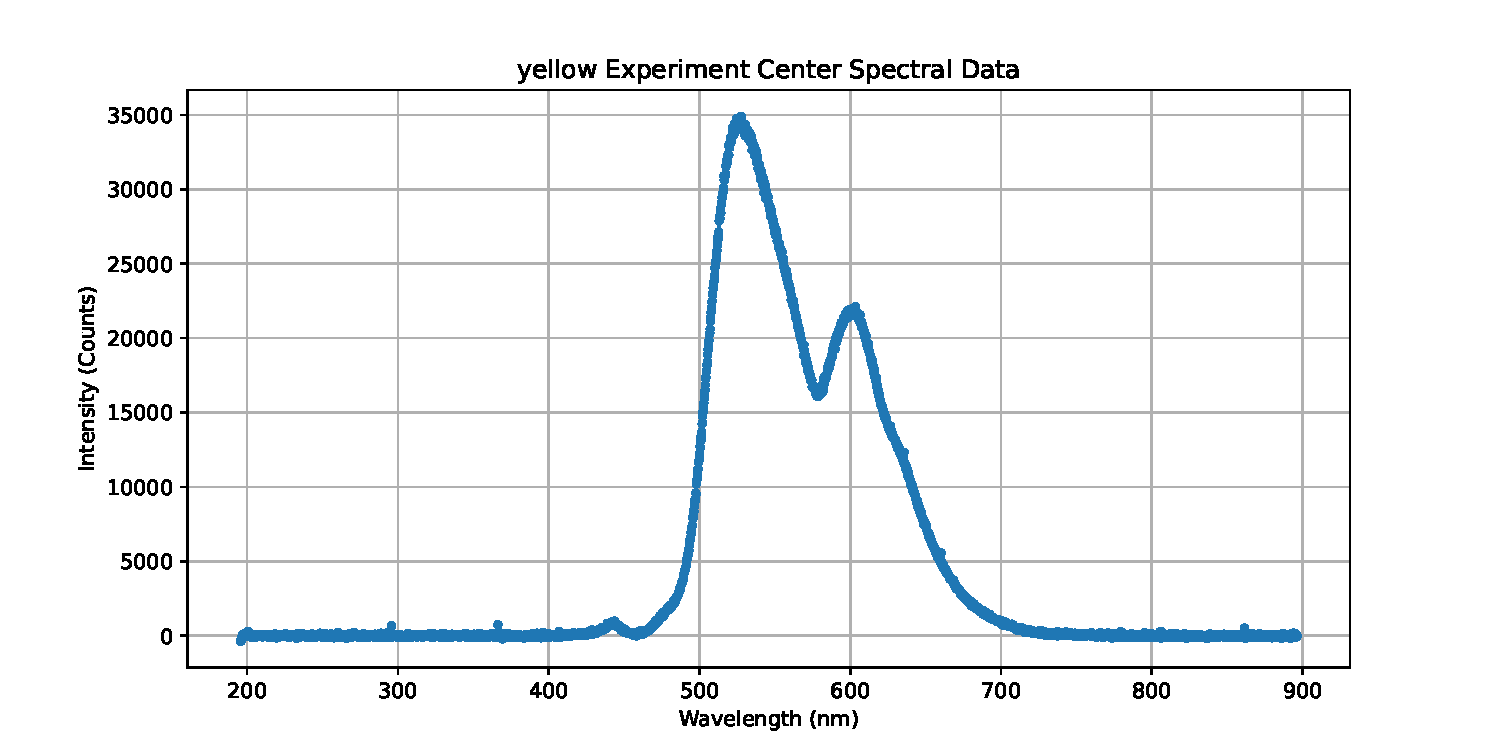
\includegraphics[keepaspectratio,width=0.6\columnwidth]{fig/yellow.pdf}
    \caption{黄色のスペクトル}
\end{figure}
\begin{figure}[htb]
    \centering
    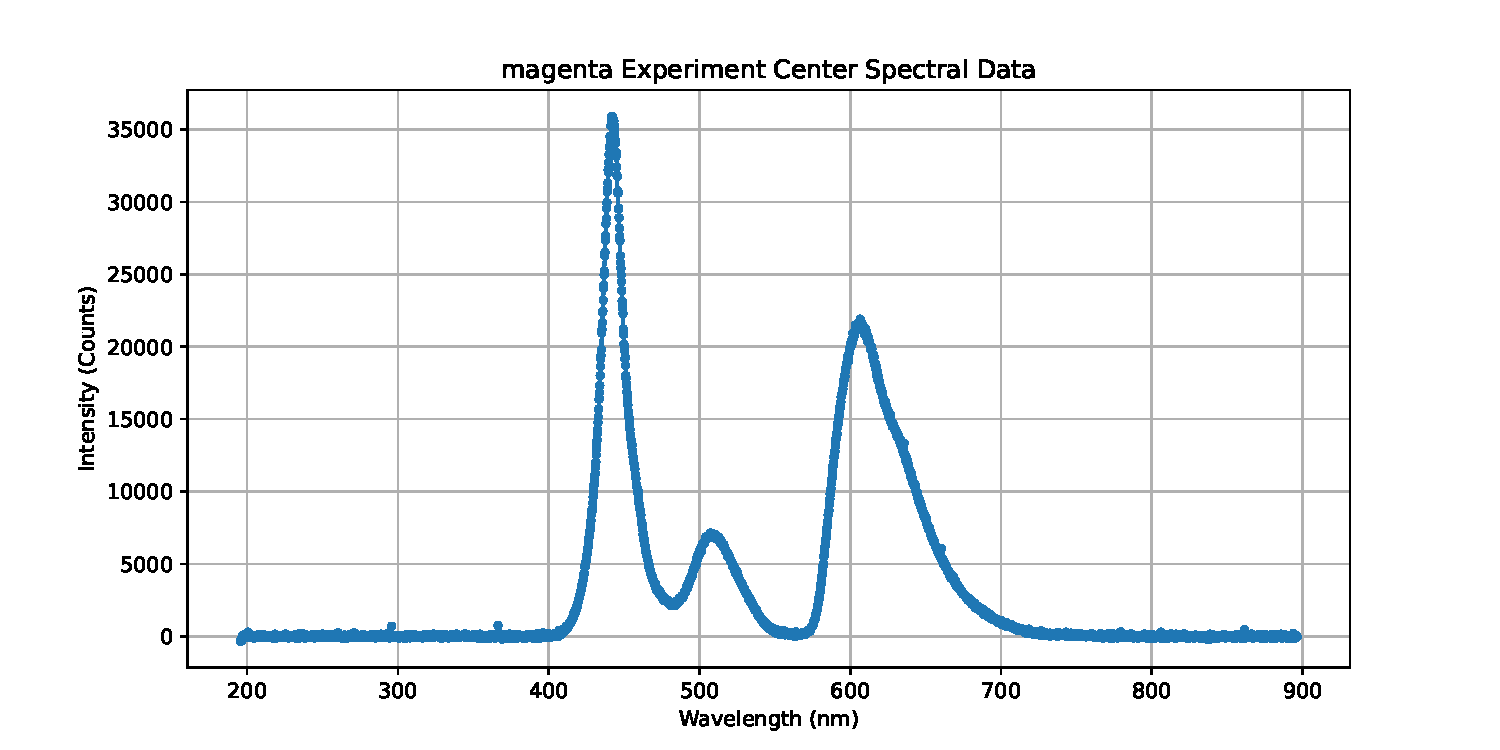
\includegraphics[keepaspectratio,width=0.6\columnwidth]{fig/magenta.pdf}
    \caption{マぜンタ(明るく鮮やかな赤紫色)のスペクトル}
\end{figure}
\begin{figure}[htb]
    \centering
    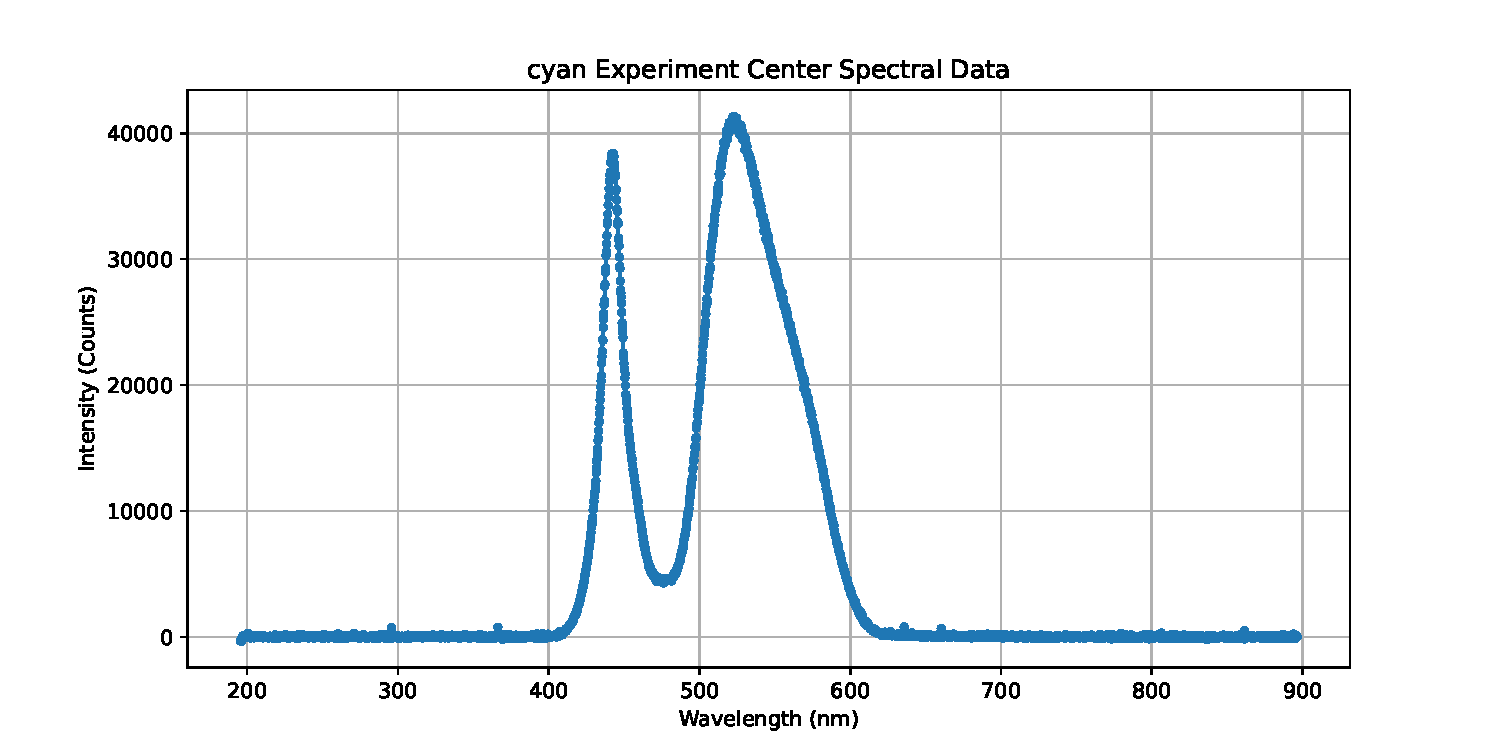
\includegraphics[keepaspectratio,width=0.6\columnwidth]{fig/cyan.pdf}
    \caption{シアン(やや緑みの明るい青)のスペクトル}
\end{figure}
\begin{figure}[htb]
    \centering
    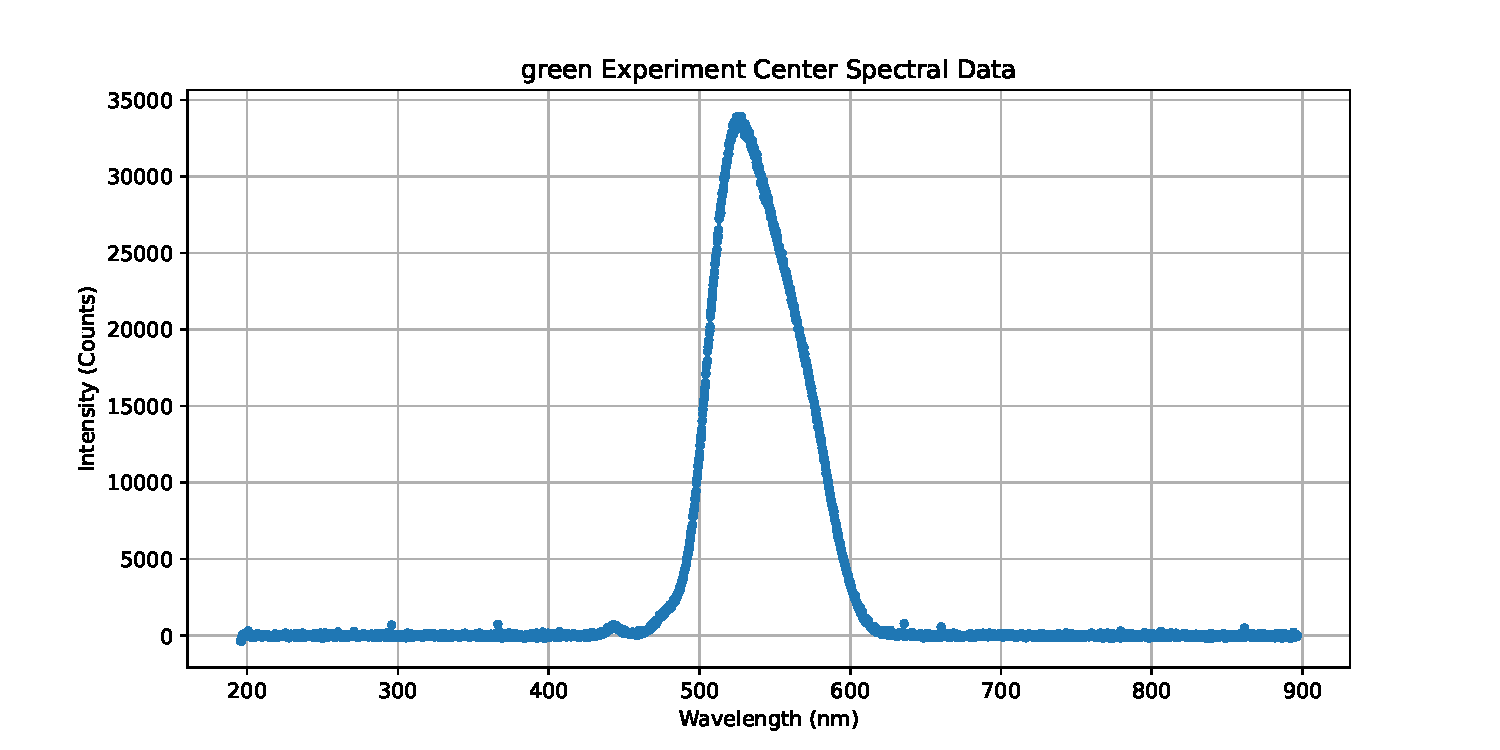
\includegraphics[keepaspectratio,width=0.6\columnwidth]{fig/green.pdf}
    \caption{緑のスペクトル}
\end{figure}
\begin{figure}[htb]
    \centering
    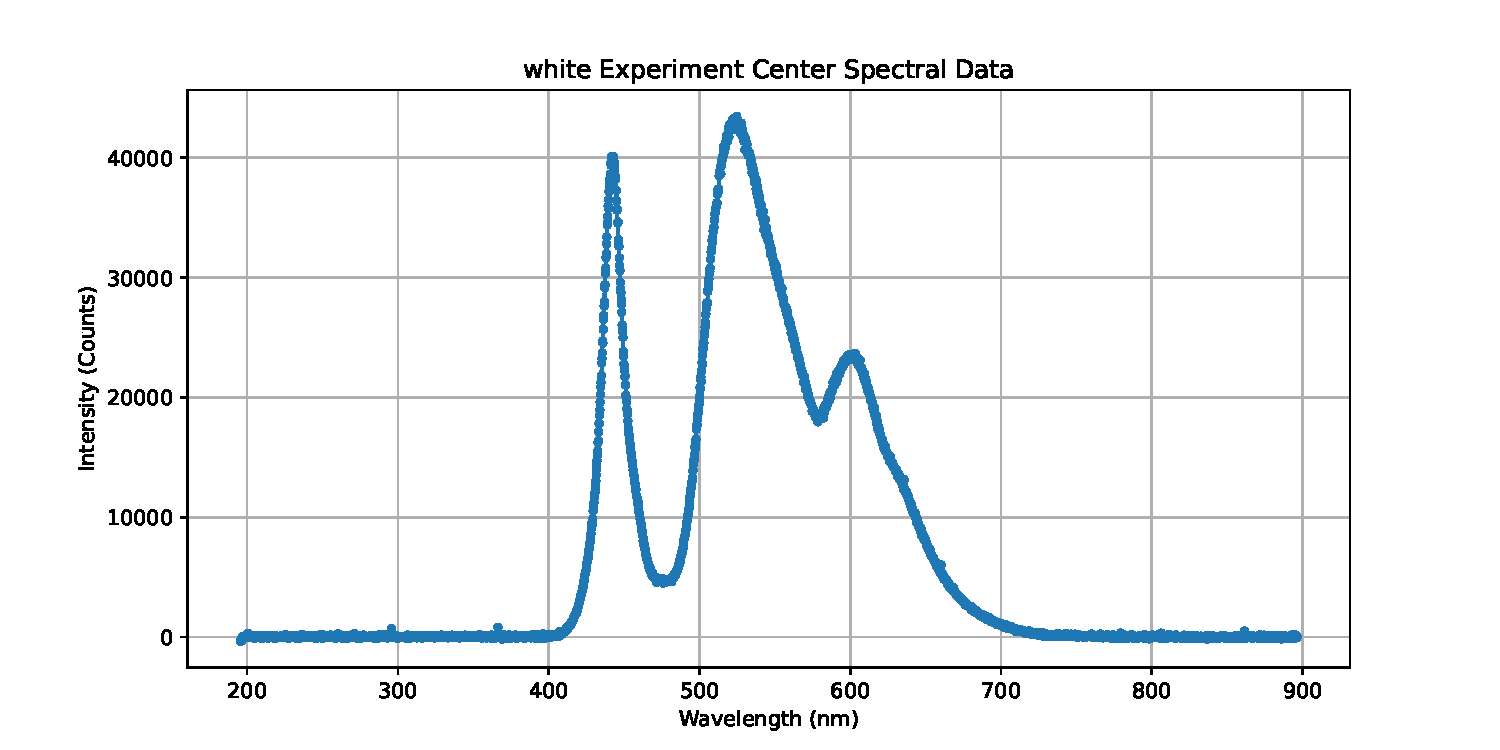
\includegraphics[keepaspectratio,width=0.6\columnwidth]{fig/white.pdf}
    \caption{白のスペクトル}
\end{figure}
\begin{figure}[htb]
    \centering
    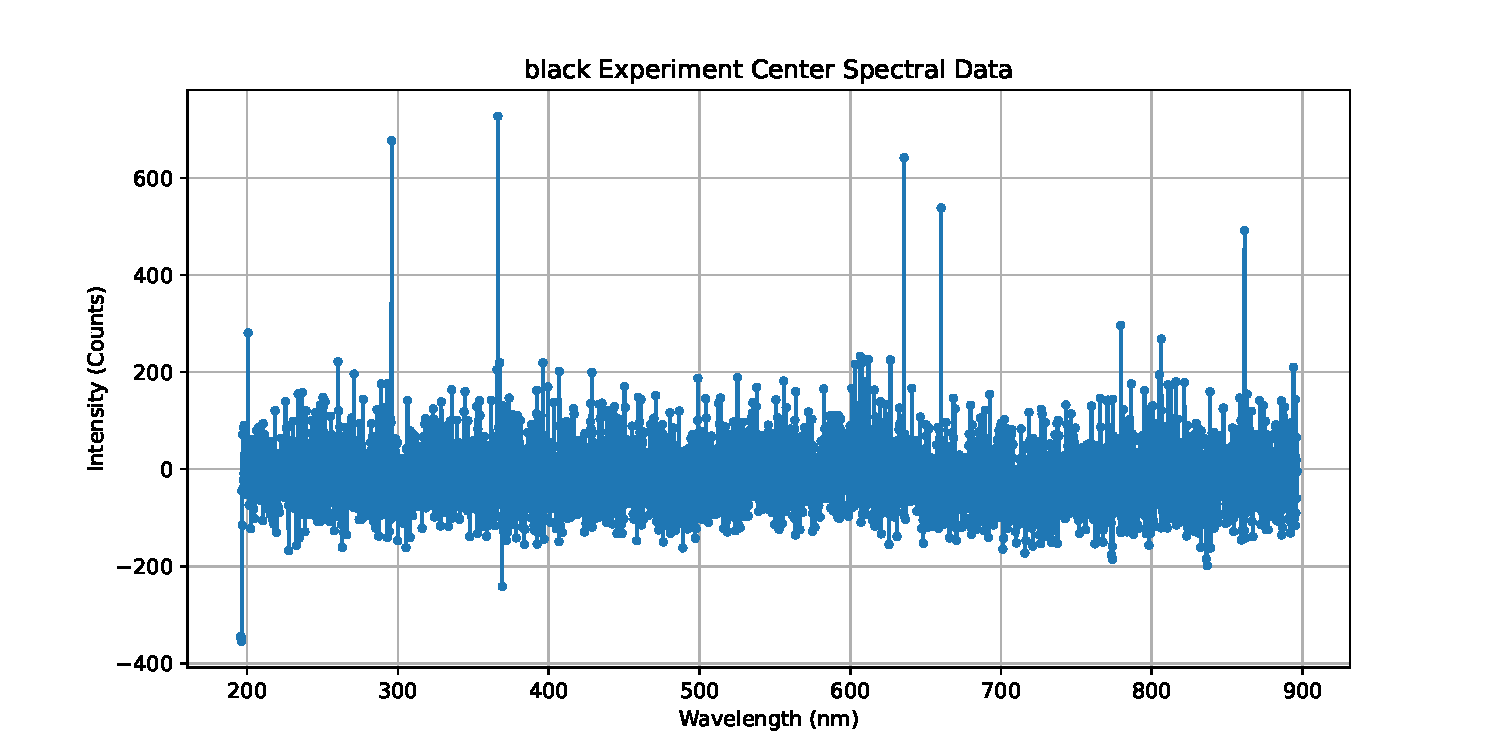
\includegraphics[keepaspectratio,width=0.6\columnwidth]{fig/black.pdf}
    \caption{黒のスペクトル}
\end{figure}

また、窒素放電管のスペクトルの300nm-400nmの部分を拡大した図を図24-25に示す。

\begin{figure}[htb]
    \centering
    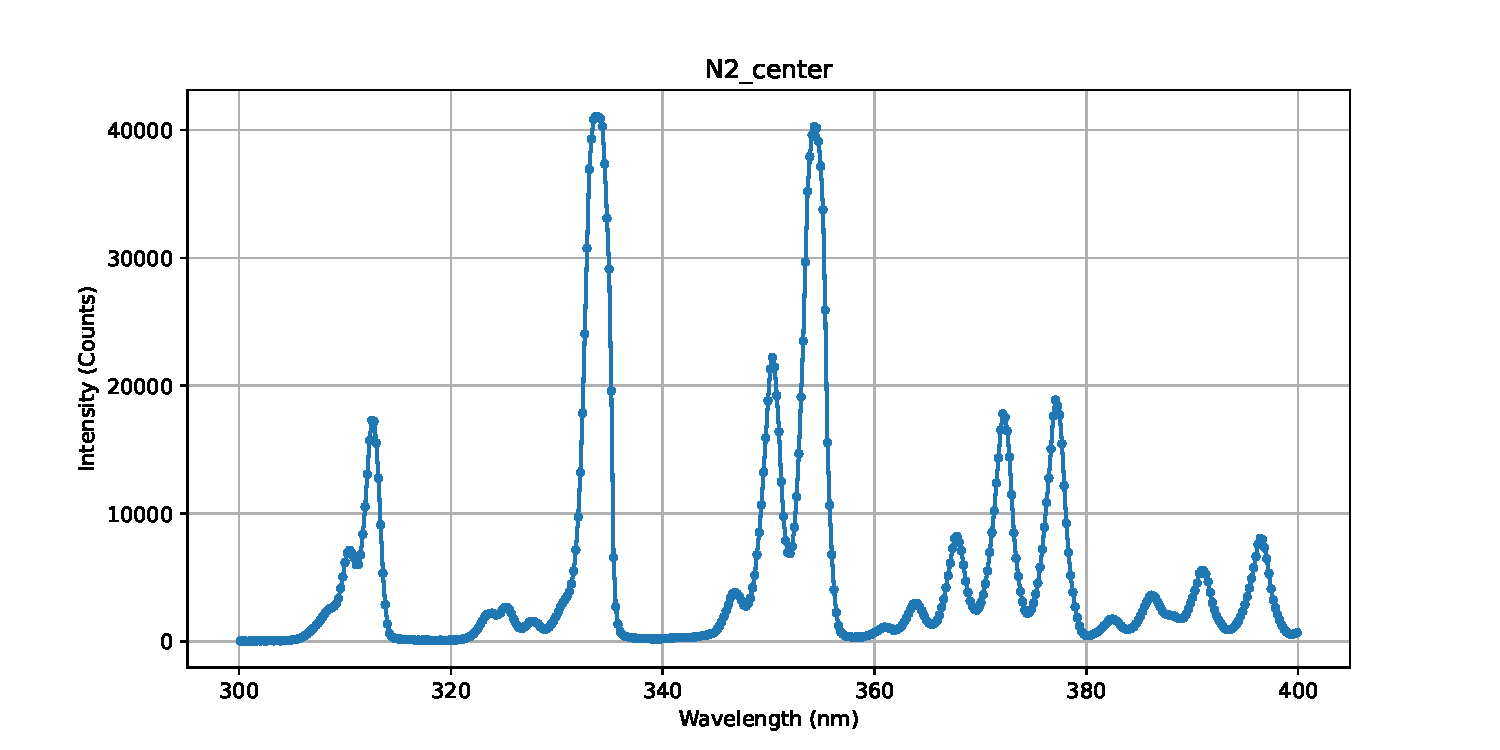
\includegraphics[keepaspectratio,width=0.6\columnwidth]{fig/N2_300-400center.pdf}
    \caption{窒素放電管の中心の300nm-400nmのスペクトル}
\end{figure}
\begin{figure}[htb]
    \centering
    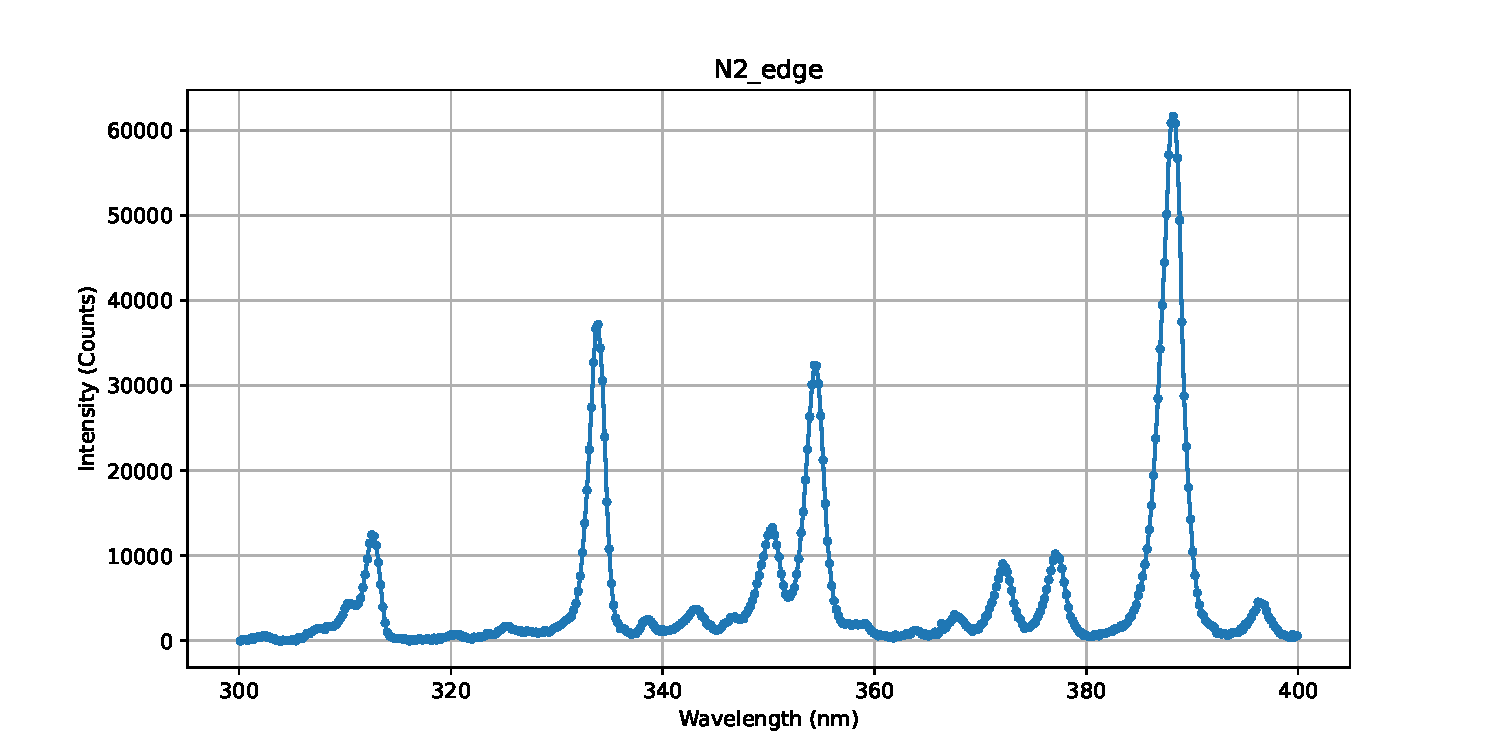
\includegraphics[keepaspectratio,width=0.6\columnwidth]{fig/N2_300-400edge.pdf}
    \caption{窒素放電管の端の300nm-400nmのスペクトル}
\end{figure}

この時、エネルギー差から波長を求めると、以下表1のようになる。
\begin{table}[htb]
    \centering
    \begin{tabular}{|c|c|}
        \hline
        \textbf{名称} & \textbf{波長 (nm)} \\
        \hline
        sp02 & 380.4 \\
        \hline
        sp13 & 375.5 \\
        \hline
        sp24 & 371.0 \\
        \hline
        sp35 & 367.0 \\
        \hline
    \end{tabular}
    \caption{波長データ}
    \label{tab:wavelengths}
\end{table}

しかし、グラフを作成するために使用した元データでは、
377.079nm, 372.123nm, 367.781nm, 363.848nmにおいてピーク値をもち、
理論波長のピーク値との差は、$3.267\pm0.115nm$の範囲にあり、$3.267nm$の誤差は、
実験中に机に触れてしまっていたこと、較正が不十分に行われていなかったことに帰因すると思われる。
また元データは、およそ0.22nm刻みであることから、$\pm0.115nm$は計測誤差の影響が大きいと推測できる。

TODO
アレニウスの式による温度計算を以下に示す。

また、波長ごとの感度を補正してからのスペクトルは図28に示す。

\begin{figure}[htb]
    \centering
    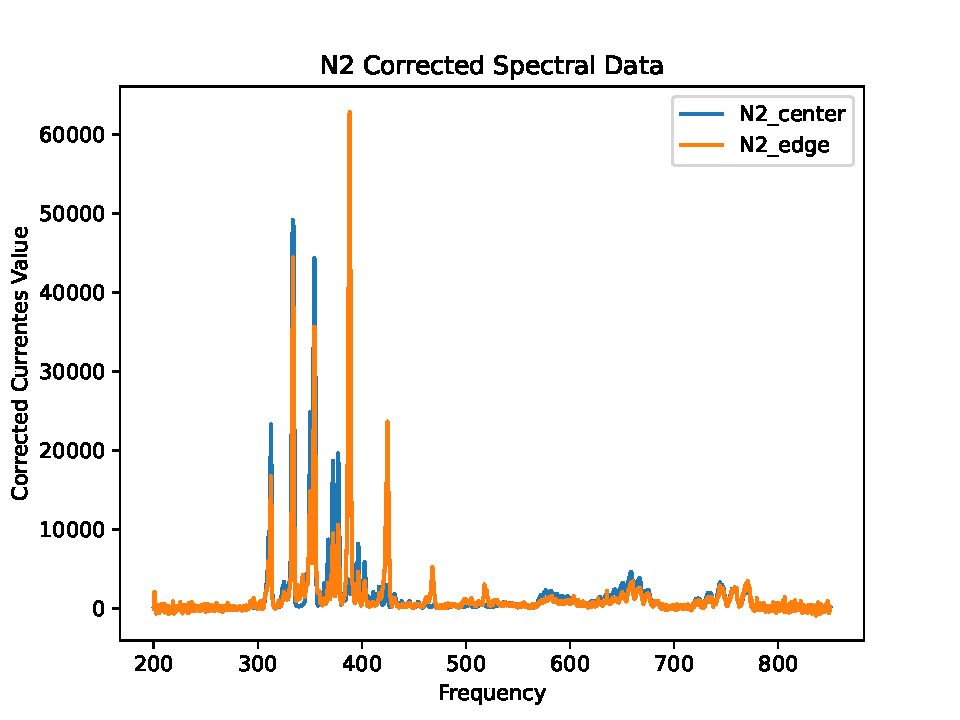
\includegraphics[keepaspectratio,width=0.6\columnwidth]{fig/hahaha.pdf}
    \caption{窒素放電管の端の300nm-400nmのスペクトル}
\end{figure}





\subsection*{水素プラズマのH原子由来のスペクトル同定}

水素原子に関してBalmer系列の $H_\alpha$,$H_\beta$,$H_\gamma$,$H_\epsilon$の発光スペクトルの波長のシミュレーション結果は表2のようになる。
$H_\alpha$,$H_\beta$,$H_\gamma$は、それぞれ9重、16重、25重の縮退となった。但し、$H_\epsilon$のデータは409.57nmのみしか出力結果に記されていなかった。
実際の波長はそれぞれ、656nm、486nm、434nm、410nmであり、シミュレーション結果と一致していることが確認できる。
しかし、シミュレーション上では、それぞれの発光スペクトルで全て同じエネルギーを取るわけではなく、それぞれのエネルギー帯の幅(微細な振動準位)を持っているかのように計算されることがわかった。


\begin{table}[h]
    \centering
    \begin{tabular}{|c|c|}
        \hline
        \textbf{名称} & \textbf{波長 (nm)} \\
        \hline
        $H_\alpha$ & 656.14, 655.48 \\
        \hline
        $H_\beta$ & 486.08, 485.66, 485.62, 485.07 \\
        \hline
        $H_\gamma$ & 433.60, 433.06, 432.58, 431.16 \\
        \hline
        $H_\epsilon$ & 409.57 \\
        \hline
    \end{tabular}
    \caption{波長データ}
\end{table}





\subsection*{He原子の発光スペクトル同定}

可視領域におけるHeの発光スペクトルのうち強度が大きい6つ(388, 447, 502, 588, 668, 707 nm 近傍)のスペクトル
はそれぞれ以下の遷移に対応する。
この時、それぞれの軌道が、どれほど縮退してるかに注意してスペクトルを帰属した。

\begin{itemize}
    \item 388nmのスペクトル: $2^3S-3^3P$
    \item 447nmのスペクトル: $2^3P-4^3D$
    \item 502nmのスペクトル: $2^1S-3^1P$
    \item 588nmのスペクトル: $2^3P-3^3D$
    \item 668nmのスペクトル: $2^1P-3^1D$
    \item 707nmのスペクトル: $2^3P-3^3S$
\end{itemize}

また、これを実験的に得られたスペクトルを比較する。
図1は、実験中の放電管の様子を示しており、放電管の端は薄ピンク色、中心は薄オレンジ色に発光した。
実際に、(388, 447, 502, 588, 668, 707 nm 近傍)のスペクトルが多く見られた。
(実験では、385,444,498,584,665,704に対応した。)
また、Heの放電菅の中心に測定素子を置いたときと、Heの放電菅の負極に測定素子を置いたときを比較すると、他のスペクトルと比べて
668nm,707nmのスペクトルに大きな変化が見られた。
TODO その理由を考察する。






\begin{figure}[htb]
    \centering
    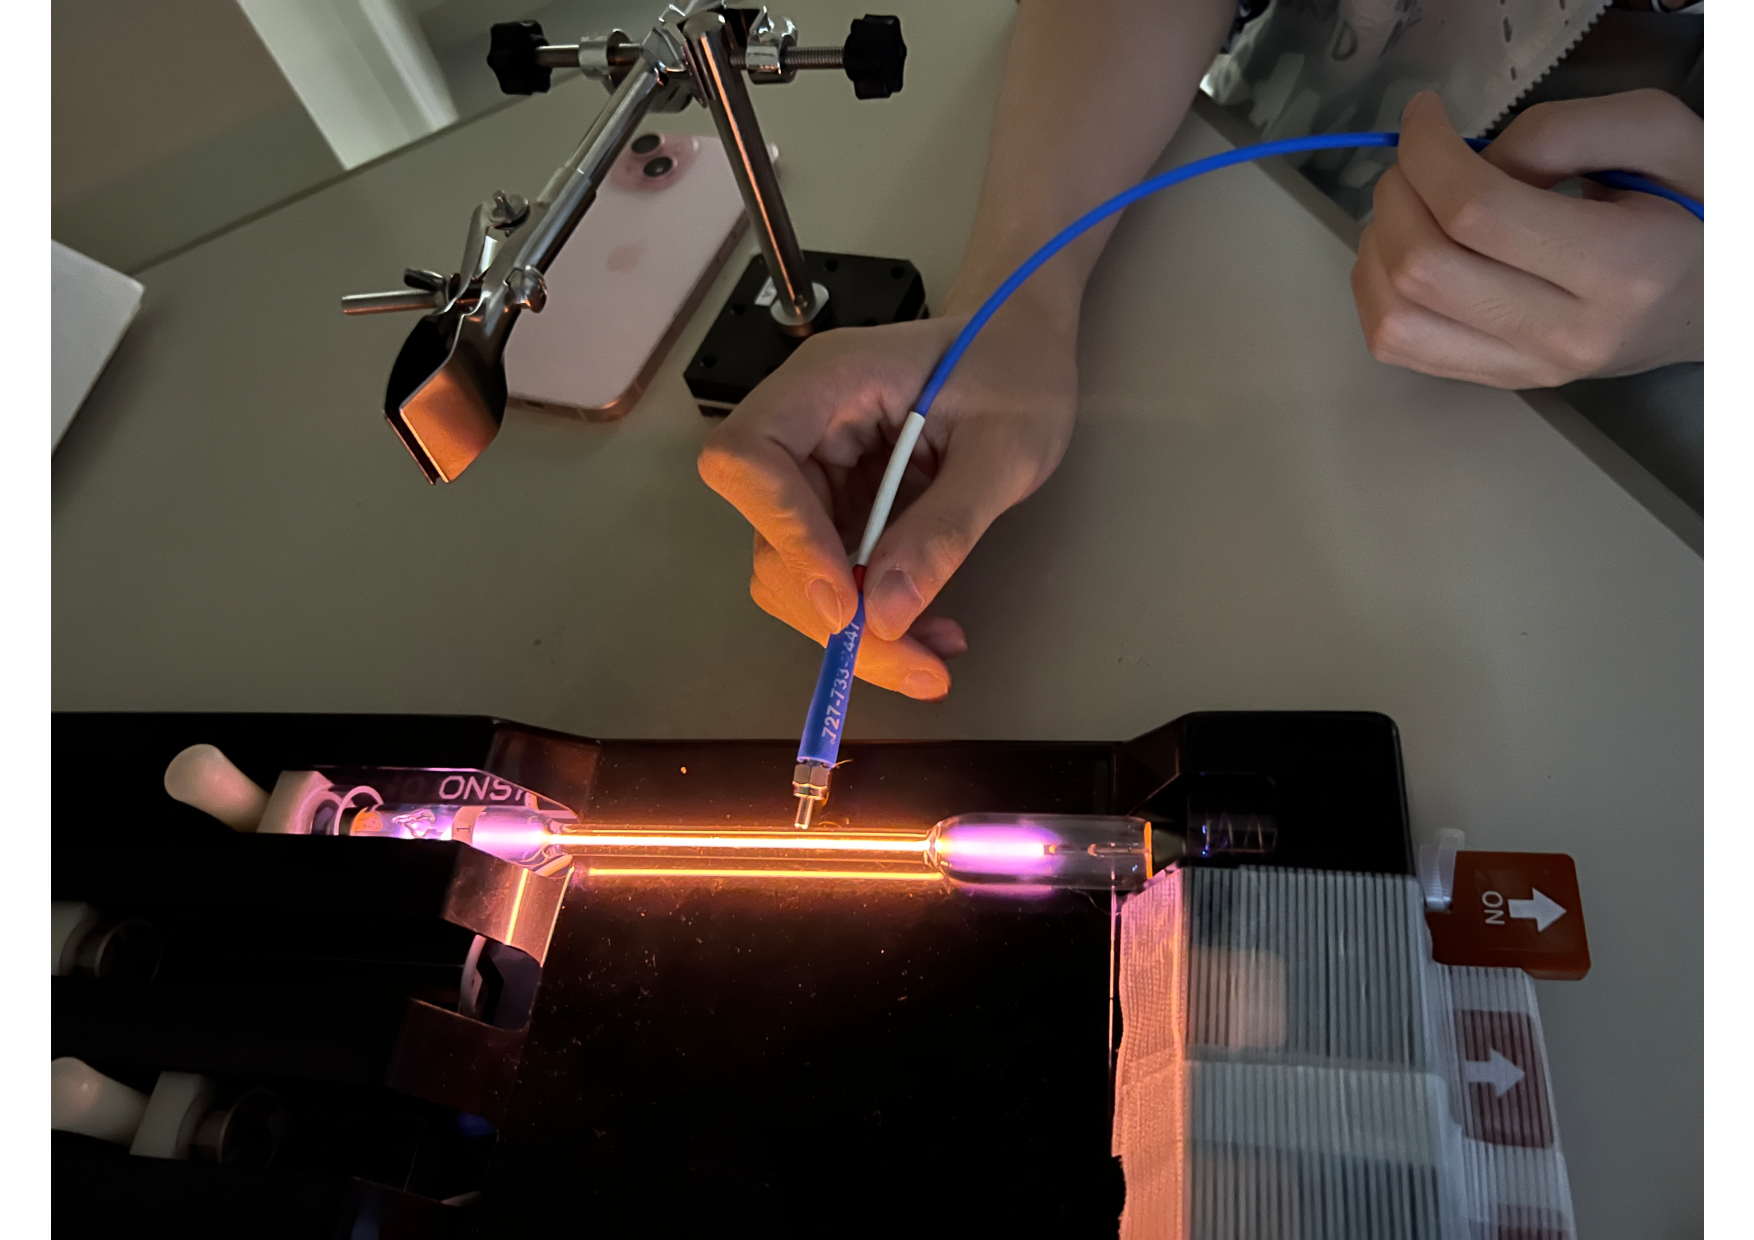
\includegraphics[keepaspectratio,width=0.6\columnwidth]{fig/latexmkrc.pdf}
    \caption{Heの放電菅の様子}
\end{figure}
\begin{figure}[htb]
    \centering
    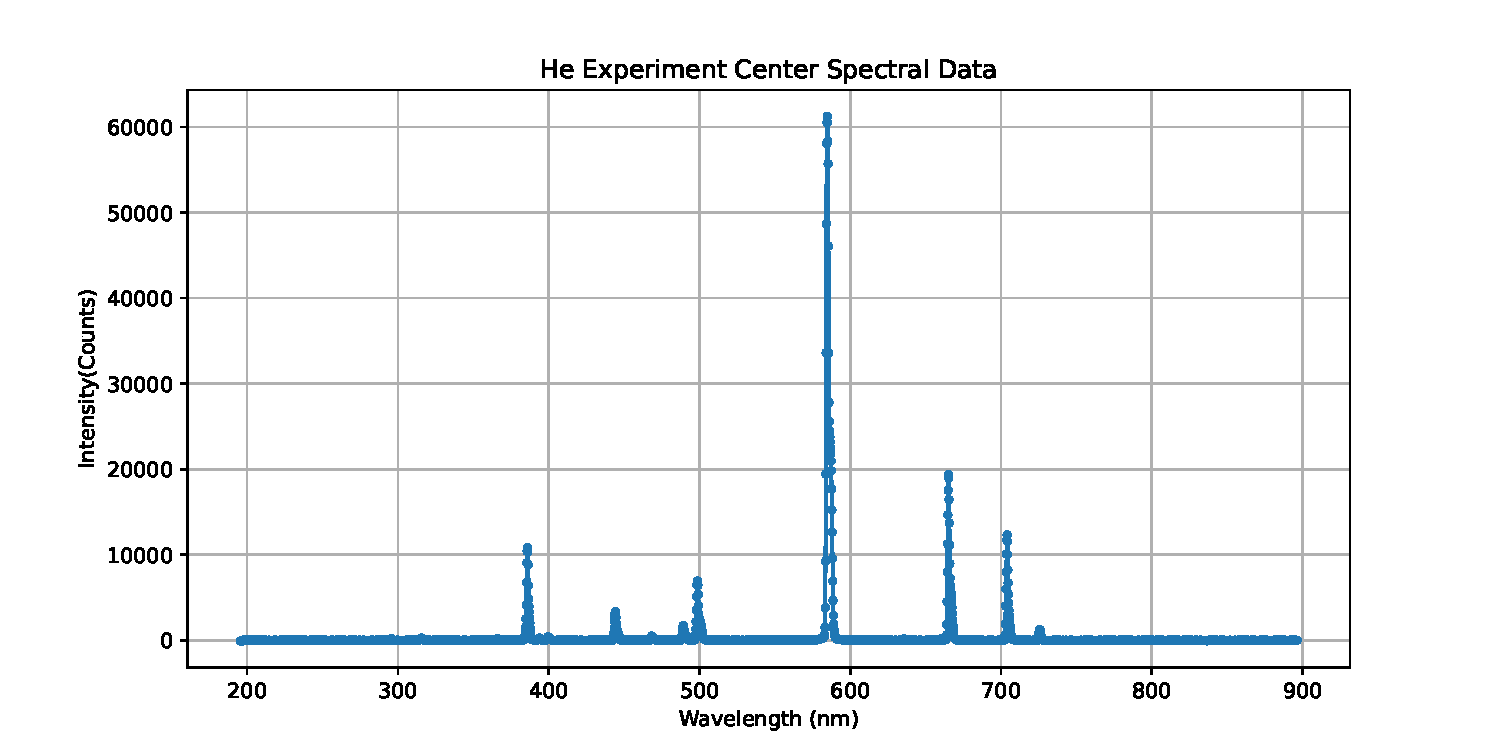
\includegraphics[keepaspectratio,width=0.6\columnwidth]{fig/He_center.pdf}
    \caption{Heの放電菅の中心に測定素子を置いたときのスペクトル}
\end{figure}
\begin{figure}[htb]
    \centering
    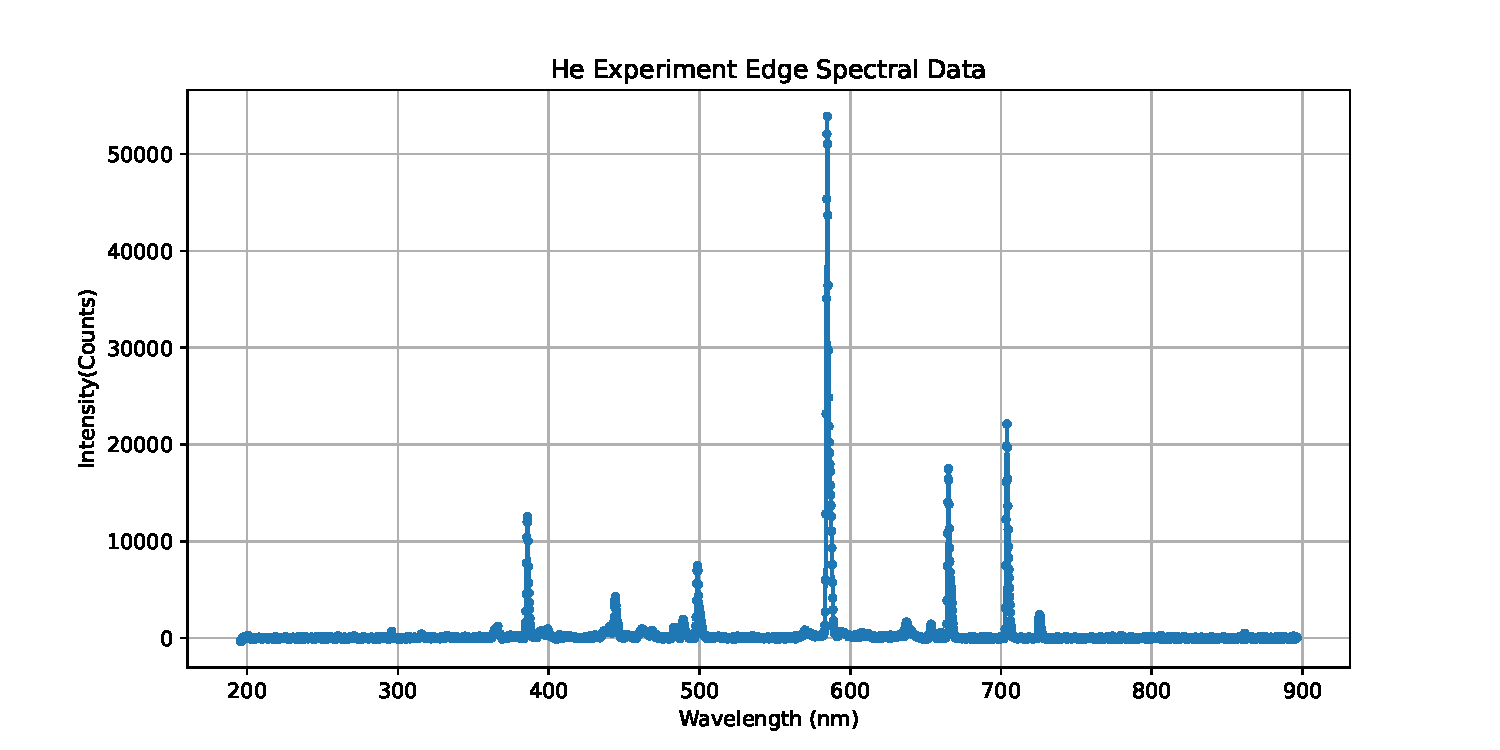
\includegraphics[keepaspectratio,width=0.6\columnwidth]{fig/He_edge.pdf}
    \caption{Heの放電菅の負極に測定素子を置いたときのスペクトル}
\end{figure}

















\bibliographystyle{junsrt}
\bibliography{cite}

\end{document}
